\documentclass[9pt]{article}

\usepackage[utf8]{inputenc}
\usepackage{geometry}
\geometry{
    a4paper,
    total={170mm,257mm},
    left=15mm,
    right=15mm,
    top=20mm,
    bottom=20mm,
}
\usepackage{multicol}
\usepackage[font=small,labelfont=bf]{caption}
\setlength{\columnsep}{0.25cm}
\usepackage[inline]{enumitem}
\usepackage{amssymb}
\usepackage{xcolor}
\usepackage{mathtools} 
\setlength{\parindent}{0em}
\setlength{\parsep}{0em}
\usepackage{tikz}
\setlength{\parskip}{0em}
\usetikzlibrary{decorations.pathmorphing,patterns}
\usepackage[american,cuteinductors]{circuitikz}
\usetikzlibrary{shapes,arrows,circuits,calc,babel}
% Definition of blocks:
\tikzset{%
  block/.style    = {draw, thick, rectangle, minimum height = 3em,
    minimum width = 3em},
  sum/.style      = {draw, circle, node distance = 2cm}, % Adder
  input/.style    = {coordinate}, % Input
  output/.style   = {coordinate} % Output
}
% Defining string as labels of certain blocks.
\newcommand{\suma}{\Large$+$}
\newcommand{\inte}{$\displaystyle \int$}
\newcommand{\derv}{\huge$\frac{d}{dt}$}

\def\mf{\ensuremath\mathbf}
\def\mb{\ensuremath\mathbb}
\def\mc{\ensuremath\mathcal}
\def\lp{\ensuremath\left(}
\def\rp{\ensuremath\right)}
\def\lv{\ensuremath\left\lvert}
\def\rv{\ensuremath\right\rvert}
\def\lV{\ensuremath\left\lVert}
\def\rV{\ensuremath\right\rVert}
\def\lc{\ensuremath\left\{}
\def\rc{\ensuremath\right\}}
\def\ls{\ensuremath\left[}
\def\rs{\ensuremath\right]}
\def\bmx{\ensuremath\begin{bmatrix*}[r]}
\def\emx{\ensuremath\end{bmatrix*}}
\def\bmxc{\ensuremath\begin{bmatrix*}[c]}
\def\emxc{\ensuremath\end{bmatrix*}}
% \def\t{\lp t\rp}
% \def\k{\ls k\rs}

\newcommand{\demoex}[2]{\onslide<#1->\begin{color}{black!60} #2 \end{color}}
\newcommand{\demoexc}[3]{\onslide<#1->\begin{color}{#2} #3 \end{color}}
\newcommand{\anim}[3]{\onslide<#1->{\begin{color}{#2!60} #3 \end{color}}}
\newcommand{\ct}[1]{\lp #1\rp}
\newcommand{\dt}[1]{\ls #1\rs}

\renewcommand{\familydefault}{\sfdefault}

\begin{document}
\begin{center}
\begin{Large}
\textbf{Linear Systems: Assignment}
\end{Large}
\end{center}
\vspace{0.2cm}

\begin{multicols}{2}

% Copyright 2004 by Till Tantau <tantau@users.sourceforge.net>.
%
% In principle, this file can be redistributed and/or modified under
% the terms of the GNU Public License, version 2.
%
% However, this file is supposed to be a template to be modified
% for your own needs. For this reason, if you use this file as a
% template and not specifically distribute it as part of a another
% package/program, I grant the extra permission to freely copy and
% modify this file as you see fit and even to delete this copyright
% notice. 

\documentclass[aspectratio=169]{beamer}
%\documentclass{beamer}

\setbeamersize{text margin left=5mm, text margin right=5mm}

\defbeamertemplate{headline}{my header}{%
\vskip1pt%
\makebox[0pt][l]{\,\insertshortauthor}%
\hspace*{\fill}\insertshorttitle/\insertshortsubtitle\hspace*{\fill}%
\llap{\insertpagenumber/\insertpresentationendpage\,}
}
\setbeamertemplate{headline}[my header]

\let\olditem\item
\renewcommand{\item}{\setlength{\itemsep}{\fill}\olditem}

\usepackage{soul}
\usepackage{tkz-euclide}
\usetikzlibrary{calc}
\usepackage[]{algorithm2e}
\usepackage{changepage}
\usepackage{amssymb}
\usepackage{xcolor}
\usepackage{mathtools}
\usepackage{tcolorbox}
\usepackage{tikz}
\usepackage{tikz-3dplot}
%\usetikzlibrary{arrows.meta}

%\setbeamertemplate{itemize items}{-}

%\usepackage{helvet}
\usefonttheme{professionalfonts} % using non standard fonts for beamer
%\usefonttheme{serif} % default family is serif
%\usepackage{fontspec}
%\setmainfont{Liberation Serif}

% There are many different themes available for Beamer. A comprehensive
% list with examples is given here:
% http://deic.uab.es/~iblanes/beamer_gallery/index_by_theme.html
% You can uncomment the themes below if you would like to use a different
% one:
%\usetheme{AnnArbor}
%\usetheme{Antibes}
%\usetheme{Bergen}
%\usetheme{Berkeley}
%\usetheme{Berlin}
%\usetheme{Boadilla}
%\usetheme{boxes}
%\usetheme{CambridgeUS}
%\usetheme{Copenhagen}
%\usetheme{Darmstadt}
%\usetheme{default}
%\usetheme{Frankfurt}
%\usetheme{Goettingen}
%\usetheme{Hannover}
%\usetheme{Ilmenau}
%\usetheme{JuanLesPins}
%\usetheme{Luebeck}
%\usetheme{Madrid}
%\usetheme{Malmoe}
%\usetheme{Marburg}
%\usetheme{Montpellier}
%\usetheme{PaloAlto}
%\usetheme{Pittsburgh}
%\usetheme{Rochester}
%\usetheme{Singapore}
%\usetheme{Szeged}
%\usetheme{Warsaw}

\def\mf{\ensuremath\mathbf}
\def\mb{\ensuremath\mathbb}
\def\lp{\ensuremath\left(}
\def\rp{\ensuremath\right)}
\def\lv{\ensuremath\left\lvert}
\def\rv{\ensuremath\right\rvert}
\def\lV{\ensuremath\left\lVert}
\def\rV{\ensuremath\right\rVert}
\def\lc{\ensuremath\left\{}
\def\rc{\ensuremath\right\}}
\def\ls{\ensuremath\left[}
\def\rs{\ensuremath\right]}
\def\bmx{\ensuremath\begin{bmatrix*}[r]}
\def\emx{\ensuremath\end{bmatrix*}}
\def\bmxc{\ensuremath\begin{bmatrix*}[c]}
\def\t{\lp t\rp}
\def\k{\ls k\rs}


\newcommand{\demoex}[2]{\onslide<#1->\begin{color}{black!60} #2 \end{color}}
\newcommand{\demoexc}[3]{\onslide<#1->\begin{color}{#2} #3 \end{color}}
\newcommand{\anim}[3]{\onslide<#1->{\begin{color}{#2!60} #3 \end{color}}}
\newcommand{\ct}[1]{\lp #1\rp}
\newcommand{\dt}[1]{\ls #1\rs}
\newcommand{\cols}[2]{\begin{columns}[#1] #2 \end{columns}}
\newcommand{\col}[2]{\begin{column}{#1} #2 \end{column}}

\title{Linear Systems}

% A subtitle is optional and this may be deleted
\subtitle{Vectors}

\author{Sivakumar Balasubramanian}
% - Give the names in the same order as the appear in the paper.
% - Use the \inst{?} command only if the authors have different
%   affiliation.

\institute[Christian Medical College] % (optional, but mostly needed)
{
  \inst{}%
  Department of Bioengineering\\
  Christian Medical College, Bagayam\\
  Vellore 632002
}
% - Use the \inst command only if there are several affiliations.
% - Keep it simple, no one is interested in your street address.

\date{}
% - Either use conference name or its abbreviation.
% - Not really informative to the audience, more for people (including
%   yourself) who are reading the slides online

\subject{Lecture notes on linear systems}
% This is only inserted into the PDF information catalog. Can be left
% out. 

% If you have a file called "university-logo-filename.xxx", where xxx
% is a graphic format that can be processed by latex or pdflatex,
% resp., then you can add a logo as follows:

% \pgfdeclareimage[height=0.5cm]{university-logo}{university-logo-filename}
% \logo{\pgfuseimage{university-logo}}

% Delete this, if you do not want the table of contents to pop up at
% the beginning of each subsection:
\AtBeginSubsection[]
{
  \begin{frame}<beamer>{Outline}
    \tableofcontents[currentsection,currentsubsection]
  \end{frame}
}

% Let's get started
\begin{document}

\begin{frame}
  \titlepage
\end{frame}

\begin{frame}[t]{References}
\begin{itemize}
\item S Boyd, Applied Linear Algebra: Chapters 1, 2, 3 and 5.
\end{itemize}
\end{frame}

\begin{frame}[t]{Vectors}
\begin{itemize}
  \item \textbf{Vectors} are ordered list of numbers (scalars). $\mathbf{v} = \begin{bmatrix*}[r] 1.2 \\ -0.1 \\ \vdots \\-1.24 \end{bmatrix*}$.\\
  \textbf{Note:} Small bold letter will represent vectors. e.g. $\mathbf{a}, \mathbf{x}, \ldots $
  
  \item Scalars can be any \textit{field} $\mathbb{R}, \mathbb{C}, \mathbb{Z}, \mathbb{Q}$. Scalars will be represented using lower case normal font, e.g. $x, y, \alpha, \beta, \ldots$
  
  \item Addition/multiplication operations performed on vectors will follow the rules of addition/multiplication of the corresponding scalar fields.
  
  \item We will typically encounter only $\mathbb{R}$ and $\mb{C}$ in this course.
\end{itemize}
\end{frame}


\begin{frame}[t]{Vectors}
\begin{itemize}
  \item Individual elements of a vector $\mathbf{v}$ are indexed. The $i^{th}$ element of $\mathbf{v}$ is referred to as $v_i$.

  \item \textit{Dimension} or \textit{size} of a vector is number of elements in the vector.
  
  \item Set of $n$-real vectors is denoted by $\mathbb{R}^n$ (similarly, $\mathbb{C}^n$)
  
  \item Vectors $\mathbf{a}$ and $\mathbf{b}$ are equal, if
  \begin{itemize}
    \item both have the same size; and
    \item $a_i = b_i, i \in \left\{1, 2, 3, \ldots n\right\}$
  \end{itemize}
  \end{itemize}
\end{frame}


\begin{frame}[t]{Vectors}
\begin{itemize}
\item \textbf{Unit vector} $\mathbf{e}_1 = \begin{bmatrix} 1 \\ 0 \\ 0 \\ \vdots \\ 0 \end{bmatrix}$ \textbf{Zero vector} $\mathbf{0} = \begin{bmatrix} 0 \\ 0 \\ 0 \\ \vdots \\ 0 \end{bmatrix}$ \textbf{One vector} $\mathbf{1} = \begin{bmatrix} 1 \\ 1 \\ 1 \\ \vdots \\ 1 \end{bmatrix}$
\item Geometrically, real $n$-vectors can be thought of as points in $\mathbb{R}^n$ space.\\
\begin{center}
\begin{tikzpicture}
\node (A) at (0,0) {$\mathbf{0}$};
\node (B) at (1,2) {$\mathbf{v}$};
\draw[thick,-latex] (A) -- (B);
\end{tikzpicture}
\end{center}
\end{itemize}
\end{frame}


\begin{frame}[t]{Vectors}
\begin{columns}[T]
\begin{column}{0.5\textwidth}
\begin{itemize}
\item \textbf{Vector scaling}: Multiplication of a scalar and a vector.
\begin{small}
$$ \mathbf{w} = a\mathbf{v} = a\begin{bmatrix} v_1 \\ v_2 \\ v_3 \\ \vdots \\ v_n \end{bmatrix} = \begin{bmatrix} av_1 \\ av_2 \\ av_3 \\ \vdots \\ av_n \end{bmatrix} \,\, a \in \mathbb{R}; \,\, \mathbf{w}, \mathbf{v} \in \mathbb{R}^n$$
\end{small}
\end{itemize}
\begin{center}
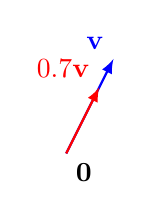
\begin{tikzpicture}[scale=0.6]
\path coordinate (a) at (0,0)
      coordinate (b) at (1.0,2.0)
      coordinate (c) at ($(a)!0.7!(b)$);
\draw[thick,blue,-latex] (a)  -> (b);
\draw[thick,red,-latex] (a)  -> (c);
\node[below right] at (a){$\mathbf{0}$}; 
\node[blue,above left] at (b){$\mathbf{v}$};
\node[red,above left] at (c){$0.7\mathbf{v}$};  
\end{tikzpicture}\hspace{1cm}
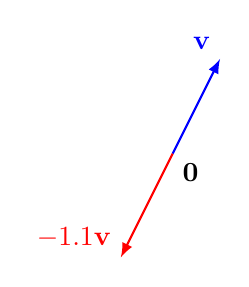
\begin{tikzpicture}[scale=0.6]
\path coordinate (a) at (0,0)
      coordinate (b) at (1.0,2.0)
      coordinate (c) at ($(a)!-1.1!(b)$);
\draw[thick,red,-latex] (a)  -> (c);
\draw[thick,blue,-latex] (a)  -> (b);
\node[below right] at (a){$\mathbf{0}$}; 
\node[blue,above left] at (b){$\mathbf{v}$};
\node[red,above left] at (c){$-1.1\mathbf{v}$};  
\end{tikzpicture}
\end{center}
\end{column}
\begin{column}{0.5\textwidth}
\textbf{Properties}
\begin{itemize}
\item Scalar multiplication is \textit{commutative}.
$$ \alpha \mathbf{v} = \mathbf{v} \alpha $$
\item Scalar multiplication is \textit{associative}.
$$ \left(\alpha \beta\right) \mathbf{v} = \alpha \left(\beta \mathbf{v}\right) $$
\item Scalar multiplication is \textit{distributive}.
$$ \left(\alpha + \beta\right) \mathbf{v} = \alpha \mathbf{v} + \beta \mathbf{v} $$
\end{itemize}
\end{column}
\end{columns}
\end{frame}


\begin{frame}[t]{Vectors}
\begin{columns}[T]
\begin{column}{0.5\textwidth}
\begin{itemize}
\item \textbf{Vector addition}: Adding two vectors of the same dimension, element by element.
\begin{small}
$$ \mathbf{u} + \mathbf{v} = \begin{bmatrix} u_1 \\ u_2 \\ u_3 \\ \vdots \\ u_n \end{bmatrix} + \begin{bmatrix} v_1 \\ v_2 \\ v_3 \\ \vdots \\ v_n \end{bmatrix}= \begin{bmatrix} u_1 + v_1 \\ u_2 + v_2 \\ u_3 + v_3 \\ \vdots \\ u_n + v_n \end{bmatrix} \,\, \mathbf{u}, \mathbf{v} \in \mathbb{R}^n$$
\end{small}
\end{itemize}
\begin{center}
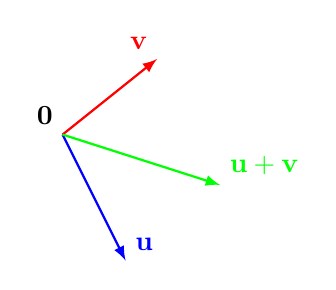
\begin{tikzpicture}[scale=0.8]
\path coordinate (a) at (0,0)
      coordinate (b) at (1.0,-2.0)
      coordinate (c) at (1.5,1.2)
      coordinate (d) at ($(b)!0.5!(c)$)
      coordinate (e) at ($(a)!2.0!(d)$);
\draw[thick,blue,-latex] (a)  -> (b);
\draw[thick,red,-latex] (a)  -> (c);
\draw[thick,green,-latex] (a)  -> (e);
\node[above left] at (a){$\mathbf{0}$}; 
\node[blue,above right] at (b){$\mathbf{u}$};
\node[red,above left] at (c){$\mathbf{v}$};
\node[green,above right] at (e){$\mathbf{u}+\mathbf{v}$};
\end{tikzpicture}
\end{center}
\end{column}
\begin{column}{0.5\textwidth}
\textbf{Properties}
\begin{itemize}
\item Vector addition is \textit{commutative}.
$$ \mathbf{a} + \mathbf{b} = \mathbf{b} + \mathbf{a} $$
\item Vector addition is \textit{associative}.
$$ \left(\mathbf{a} + \mathbf{b}\right) + \mathbf{c} =  \mathbf{a} + \left(\mathbf{b} + \mathbf{c} \right) $$
\item Zero vector has no effect.
$$ \mathbf{a} + \mathbf{0} = \mathbf{a} $$
\item Subtraction of vectors. 
$$ \mathbf{a} + (-1)\mathbf{a} = \mathbf{a} - \mathbf{a} = \mathbf{0} $$
\end{itemize}
\end{column}
\end{columns}
\end{frame}


\begin{frame}[t]{Vector spaces}
\begin{itemize}
\item A set of vectors $V$ that is closed under \textbf{vector addition} and \textbf{vector scaling}.
\[  \forall \mathbf{x}, \mathbf{y} \in V, \,\,\,\, \mathbf{x} + \mathbf{y} \in V \]
\[  \forall \mathbf{x} \in V, \,\,\, \mathrm{and} \,\,\, \alpha \in F, \,\,\,\, \alpha \mathbf{x} \in V \]
\item For a set to be a vector space, it must satisfy the followng properties: $\mathbf{x}, \mathbf{y}, \mathbf{z} \in V$
\begin{itemize}
\item \textit{Commutativity}: $\mathbf{x} + \mathbf{y} = \mathbf{y} + \mathbf{x}$
\item \textit{Associativity of vector addition}: $(\mathbf{x} + \mathbf{y}) + \mathbf{z} = \mathbf{x} + (\mathbf{y} + \mathbf{z})$
\item \textit{Additive identity}: $\mathbf{x} + \mathbf{0} = \mathbf{0} + \mathbf{x} = \mathbf{x}$ $\left(0 \in V\right)$
\item \textit{Additive inverse}: $\exists -\mathbf{x} \in V, \mathbf{x} + (-\mathbf{x}) = \mathbf{0}$
\item \textit{Associativity of scalar multiplication}: $\alpha\left(\beta \mathbf{x}\right) = \left(\alpha\beta \mathbf{x}\right)$
\item \textit{Distributivity of scalar sums}: $\left(\alpha + \beta\right)\mathbf{x} = \alpha \mathbf{x} + \beta \mathbf{x}$
\item \textit{Distributivity of vector sums}: $\alpha\left(\mathbf{x} + \mathbf{y}\right) = \alpha \mathbf{x} + \alpha \mathbf{y}$
\item \textit{Scalar multiplication identity}: $1\mathbf{x} = \mathbf{x}$
\end{itemize}
\item We will mostly deal with $\mathbb{R}^n$ and $\mb{C}^n$ vectors spaces in this course.
\end{itemize}
\end{frame}

\begin{frame}[t]{Subspaces}
\begin{itemize}
    \item A \textbf{subspace} $S$ of a vector space $V$ is a subset of $V$ and is itself a vector space.
    \[ S \subset V, \,\,\,\, \forall \mathbf{x}, \mathbf{y} \in S, \alpha \mathbf{x} + \beta \mathbf{y} \in S, \,\,\, \alpha, \beta \in F \]
    \item The zero vector is called the \textbf{trivial subspace} of a vector space $V$.
    \item For example, in $\mathbb{R}^3$ all planes and lines passing through the origin are subspaces of $\mathbb{R}^3$. 
\end{itemize}
\begin{center}
\tdplotsetmaincoords{70}{110}
\begin{tikzpicture}[scale=2,tdplot_main_coords]
    \def\x{.75}
    \filldraw[draw=white, fill=blue!20] (\x, 0, \x)-- (\x, 0, {-1*\x})-- ({-1*\x}, 0, {-1*\x})-- ({-1*\x}, 0, \x)-- cycle;
    \draw[thick,-latex] (0,0,0) -- (1.5,0,0) node[anchor=north east]{$x$};
    \draw[thick,-latex] (0,0,0) -- (0,1,0) node[anchor=north west]{$y$};
    \draw[thick,-latex] (0,0,0) -- (0,0,1) node[anchor=south]{$z$};
    \draw[thin,dashed] (0,0,0) -- (-0.75,0,0);
    \draw[thin,dashed] (0,0,0) -- (0,-0.5,0);
    \draw[thin,dashed] (0,0,0) -- (0,0,-0.5);

    \draw[thick, red, -] (-1,-1,0) -- (1,1,0);
\end{tikzpicture}
\end{center}
\end{frame}


\begin{frame}[t]{Linear independence}
\begin{itemize}
  \item A collection of vectors $\left\{\mathbf{x}_1, \mathbf{x}_2, \mathbf{x}_3, \ldots \mathbf{x}_n\right\}, \,\,\, \mathbf{x}_i \in \mathbb{R}^m \,\,\, i \in\left\{1, 2, 3, \ldots n\right\}$ is called \textit{linearly dependent} if,
  $$ \sum_{i=1}^n\alpha_i\mathbf{x}_i = 0, \text{ hold for some } \alpha_1, \alpha_2, \ldots \alpha_n \in \mathbb{R}, \text{ such that } \exists \alpha_i \neq 0 $$
  
  \item Another way to state this: A collection of vectors is \textit{linearly dependent} if at least one of the vectors in the collection can be expressed as a linear combination of the other vectors in the collection, i.e.
  $$\mathbf{x}_i = -\sum_{j=1, j\neq i}^{n}\left(\frac{\alpha_j}{\alpha_i}\right)\mathbf{x}_j$$
  
  \item A collection of vectors is \textit{linearly independent} if it is \textbf{not} \textit{linearly dependent}.
  $$ \sum_{i=1}^n\alpha_i\mathbf{x}_i = 0 \implies \alpha_1=\alpha_2=\alpha_3\ldots=\alpha_n = 0$$
\end{itemize}
\end{frame}

\begin{frame}[t]{Span of a set of vectors}
\begin{itemize}
    \item Consider a set of vectors $S = \left\{\mathbf{v}_1, \mathbf{v}_2, \mathbf{v}_3 \ldots \mathbf{v}_r\right\}$ where $\mathbf{v}_i \in \mathbb{R}^n, 1 \leq i \leq r$.
    \item The \textbf{span} of the set $S$ is defined as the set of all linear combination of the vectors $\mathbf{v}_i$,
    \[ span\left(S\right) = \left\{\alpha_1\mathbf{v}_1 = \alpha_2\mathbf{v}_2 + \ldots + \alpha_r\mathbf{v}_r\right\}, \,\, \alpha_i \in \mathbb{R} \]
    \item Is $span\left(S\right)$ a subspace of $\mathbb{R}^n$?
    \item We say that the subspace $span\left(S\right)$ is spanned by the \textit{spanning set} $S$. $\longrightarrow$ $S$ \textit{spans} $span\left(S\right)$.
    \item \textbf{Sum of subspaces} $X, Y$ is defined as the sum of all possible vectors from $X$ and $Y$.
    \[ X + Y = \left\{\mathbf{x} + \mathbf{y} \left|\right. \mathbf{x} \in X, \mathbf{y} \in Y\right\} \]
    \item Sum of two subspace is also a subspace.
\end{itemize}
\end{frame}


\begin{frame}[t]{Inner Product}
\begin{itemize}
    \item \textbf{Standard inner product} is defined as the following,
    $$\mathbf{x}^T\mathbf{y} = \sum_{i=1}^{n}x_iy_i, \,\,\, \mathbf{x}, \mathbf{y} \in \mathbb{R}^n$$\\
    For complex vectors:  $\mathbf{x}^{*}\mathbf{y} = \sum_{i=1}^{n}\overline{x}_iy_i, \,\,\, \mathbf{x}, \mathbf{y} \in \mathbb{C}^n$
    \item \textbf{Properties}
    \begin{itemize}
        \item $\mathbf{x}^T\mathbf{x} > 0, \,\,\, \forall \mathbf{x} \neq 0$ and $\mathbf{x}^T\mathbf{x} = 0 \Leftrightarrow \mathbf{x} = 0$
        \item \textit{Commutative}: $\mathbf{x}^T\mathbf{y} = \mathbf{y}^T\mathbf{x}$
        \item \textit{Associativity with scalar multiplication}: $\left(\alpha \mathbf{x}\right)^T\mathbf{y} = \alpha \left(\mathbf{x}^T\mathbf{y}\right)$
        \item \textit{Distributivity with vector addition}: $\left(\mathbf{x} + \mathbf{y}\right)^T\mathbf{z} = \mathbf{x}^T\mathbf{z} + \mathbf{y}^T\mathbf{z}$
    \end{itemize}
\end{itemize}
\end{frame}


\begin{frame}[t]{Norm}
\begin{columns}[T]
\begin{column}{0.65\textwidth}
\vspace{-0.5cm}
\begin{small}
\begin{itemize}
  \item Norm is a measure of the size of a vector.
  \item \textit{Euclidean norm} of a $n$-vector $\mathbf{x} \in \mathbb{R}^n$ is defined as, $\left\Vert \mathbf{x}\right\Vert_2 = \sqrt{\mathbf{x}^T\mathbf{x}} = \sqrt{\sum_{i=1}^{n}x_i^2}$.
  \item $\left\Vert \mathbf{x} \right\Vert_2$ is a measure of the length of the vector $\mathbf{x}$.
  \item Any function of the form $\left\Vert\bullet\right\Vert: \mathbb{R}^n \longrightarrow \mathbb{R}_{\geq 0}$ is a valid norm, provided it satisfies the following properties.
  \item \textbf{Properties}
  \begin{itemize}
  \item \textit{Definiteness}. $\left\Vert \mathbf{x}\right\Vert = 0 \iff x = 0$
  \item \textit{Non-negativity}. $\left\Vert \mathbf{x} \right\Vert \geq 0$
  \item \textit{Non-negative homogeneity}. $\left\Vert \beta \mathbf{x} \right\Vert = \left|\beta\right|\left\Vert \mathbf{x} \right\Vert, \, \beta \in \mathbb{R}$
  \item \textit{Triangle inequality}. $\left\Vert \mathbf{x} + \mathbf{y}\right\Vert \leq \left\Vert \mathbf{x}\right\Vert + \left\Vert \mathbf{y}\right\Vert$
  \end{itemize}
  \item $p$-norm: $\left\Vert \mathbf{x} \right\Vert_p = \left(\sum_{i=1}^{n}\left|x_i\right|^p\right)^{\frac{1}{p}}$
  \item Norm of difference between two vectors is a measure of the distance between the vectors. $d = \left\Vert \mathbf{x} - \mathbf{y} \right\Vert_2$.
\end{itemize}
\end{small}
\end{column}
\begin{column}{0.35\textwidth}
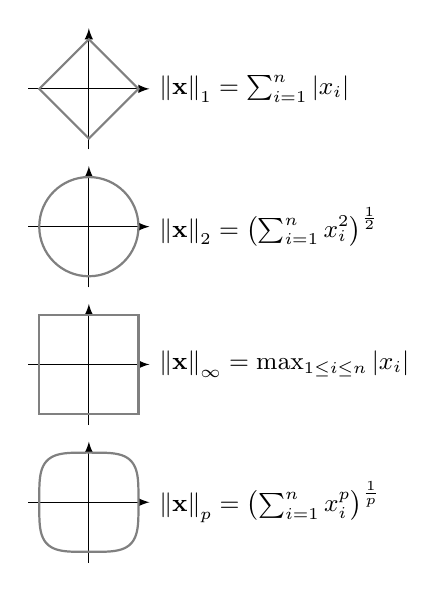
\begin{tikzpicture}[scale=0.7]
  \def \r{0.9}
  \def \ya{0}
  \def \yb{-2.5}
  \def \yc{-5}
  \def \yd{-7.5}
  
  \draw[-latex] (3.9,\ya) -- (6.1,\ya) node[black,right,xshift=0.cm, yshift=0.cm] {\small{$\left\Vert \mathbf{x} \right\Vert_1 = \sum_{i=1}^{n}\left|x_i\right|$}};
  \draw[-latex] (5,\ya-1.1) -- (5,\ya+1.1);
  \draw[thick, gray] (5-\r,0)--(5,\r)--(5+\r,0)--(5,-\r)--cycle;
  
  \draw[-latex] (3.9,\yb) -- (6.1,\yb) node[black,right,xshift=0.cm, yshift=0.cm] {\small{$\left\Vert \mathbf{x} \right\Vert_2 = \left(\sum_{i=1}^{n}x_i^2\right)^{\frac{1}{2}}$}};
  \draw[-latex] (5,\yb-1.1) -- (5,\yb+1.1);
  \draw [thick, gray](5,-2.5) circle (\r);
  
  \draw[-latex] (3.9,\yc) -- (6.1,\yc) node[black,right,xshift=0.cm, yshift=0.cm] {\small{$\left\Vert \mathbf{x} \right\Vert_\infty = \max_{1\leq i\leq n}\left|x_i\right|$}};
  \draw[-latex] (5,\yc-1.1) -- (5,\yc+1.1);
  \draw[thick, gray] (5-\r,-5-\r)--(5-\r,-5+\r)--(5+\r,-5+\r)--(5+\r,-5-\r)--cycle;

  \draw[-latex] (3.9,\yd) -- (6.1,\yd) node[black,right,xshift=0.cm, yshift=0.cm] {\small{$\left\Vert \mathbf{x} \right\Vert_p = \left(\sum_{i=1}^{n}x_i^p\right)^{\frac{1}{p}}$}};
  \draw[-latex] (5,\yd-1.1) -- (5,\yd+1.1);
  \draw[thick, gray,scale=1,domain=0:90,samples=100,smooth,variable=\t]
  plot({-\r*sqrt(cos(\t))+5},{\r*sqrt(sin(\t))-7.5});
  \draw[thick, gray,scale=1,domain=0:90,samples=100,smooth,variable=\t]
  plot({-\r*sqrt(cos(\t))+5},{-\r*sqrt(sin(\t))-7.5});
  \draw[thick, gray,scale=1,domain=0:90,samples=100,smooth,variable=\t]
  plot({\r*sqrt(cos(\t))+5},{-\r*sqrt(sin(\t))-7.5});
  \draw[thick, gray,scale=1,domain=0:90,samples=100,smooth,variable=\t]
  plot({\r*sqrt(cos(\t))+5},{\r*sqrt(sin(\t))-7.5});                 
\end{tikzpicture}
\end{column}
\end{columns}
\end{frame}


\begin{frame}[t]{Orthogonality}
\begin{itemize}
\item Orthogonality is the idea of two vectors being perpendicular, $\mathbf{x} \perp \mathbf{y}$.
\begin{center}
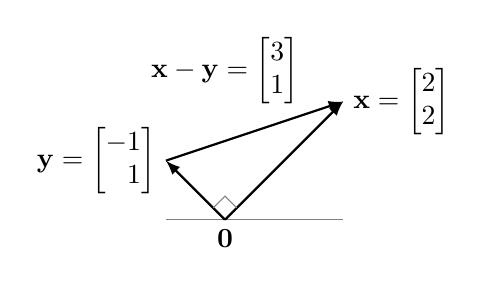
\begin{tikzpicture}[scale=0.75]
  \node[black, below] at (0, 0) {$\mathbf{0}$};
  \draw[gray,thin,-] (-1, 0) -- (2, 0) ;
  \draw[black,thick,-latex] (0, 0) -- (2, 2) node[black, above, right]{$\mathbf{x}=\begin{bmatrix*}[r]2\\2\end{bmatrix*}$};
  \draw[black,thick,-latex] (0, 0) -- (-1, 1) node[black, above, left]{$\mathbf{y}=\begin{bmatrix*}[r]-1\\1\end{bmatrix*}$};
  \draw[black,thick,-latex] (-1, 1) -- (2, 2) node[black, yshift=0.40cm, xshift=-1.5cm]{$\mathbf{x}-\mathbf{y}=\begin{bmatrix*}[r]3\\1\end{bmatrix*}$};
  \draw [gray,thin](0.2,0.2) -- (0, 0.4) -- (-0.2, 0.2);
\end{tikzpicture}
\end{center}

Using the Pythagonean theorem,  $\left\lVert \mathbf{x} - \mathbf{y}\right\rVert^2 = \left\lVert \mathbf{x}\right\rVert^2 + \left\lVert \mathbf{y}\right\rVert^2$
\[ \left\lVert \mathbf{x}\right\rVert^2 + \left\lVert \mathbf{y}\right\rVert^2 - 2 \mathbf{x}^T\mathbf{y} = \left\lVert \mathbf{x}\right\rVert^2 + \left\lVert \mathbf{y}\right\rVert^2 \implies \mathbf{x}^T\mathbf{y} = 0 \]

\item We extend this to the $n$-dimensional case and define two vectors $\mathbf{x}, \mathbf{y} \in \mathbb{R}^n$ being orthogonal, if
\[ \mathbf{x}^T\mathbf{y} = \sum_{i=1}^{n}x_iy_i = 0\]
\end{itemize}
\end{frame}


\begin{frame}[t]{Angle between vectors}
\vspace{-0.5cm}
\begin{center}
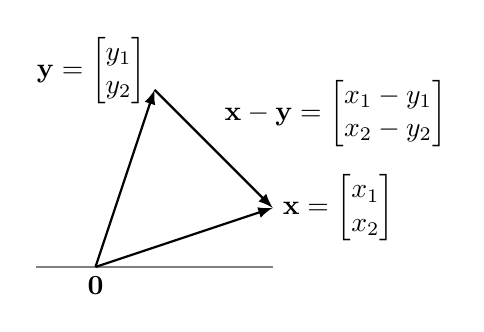
\begin{tikzpicture}[scale=0.75]
  \node[black, below] at (0, 0) {$\mathbf{0}$};
  \draw[gray,thin,-] (-1, 0) -- (3, 0) ;
  \draw[black,thick,-latex] (0, 0) -- (3, 1) node[black, above, right]{$\mathbf{x} = \begin{bmatrix*}x_1\\x_2\end{bmatrix*}$};
  \draw[black,thick,-latex] (0, 0) -- (1, 3) node[black, yshift=0.25cm, xshift=-0.8cm]{$\mathbf{y} = \begin{bmatrix*}y_1\\y_2\end{bmatrix*}$};
  \draw[black,thick,-latex] (1, 3) -- (3, 1) node[black, xshift=0.8cm, yshift=1.2cm]{$\mathbf{x} - \mathbf{y} = \begin{bmatrix*}x_1-y_1\\x_2-y_2\end{bmatrix*}$};
  % \draw[gray,domain=20:70] plot({0.75 * cos(\x)}, {0.75 * sin(\x)});
  % \node[gray, below] at (0.75, 1.0) {{\footnotesize $\theta$}};
  % \draw[blue,domain=0:19] plot({1.0 * cos(\x)}, {1.0 * sin(\x)});
  % \node[blue, yshift=0.15cm] at (1.3, 0.0) {{\footnotesize $\beta$}};
  % \draw[red,domain=0:70] plot({0.5 * cos(\x)}, {0.5 * sin(\x)});
  % \node[red, yshift=0.18cm] at (0.23, 0.0) {{\footnotesize $\alpha$}};
  % \node[right] at (7,3.5) {$\cos \alpha = \frac{y_1}{\left\lVert \mathbf{y}\right\rVert}, \,\,\, \cos \beta = \frac{x_1}{\left\lVert \mathbf{x}\right\rVert}$};
  % \node[right] at (7,2.5) {$\sin \alpha = \frac{y_2}{\left\lVert \mathbf{y}\right\rVert}, \,\,\, \sin \beta = \frac{x_2}{\left\lVert \mathbf{x}\right\rVert}$};
  % \node[right] at (7,1.5) {$\cos \left(\alpha - \beta\right) = \cos \alpha \cos \beta + \sin \alpha \cos \beta$};
  % \node[right] at (7,0.5) {$\cos \left(\theta\right) = \frac{x_1y_1 + x_2y_2}{\left\lVert \mathbf{x}\right\rVert \left\lVert \mathbf{y}\right\rVert} = \frac{\mathbf{x}^T\mathbf{y}}{\left\lVert \mathbf{x}\right\rVert \left\lVert \mathbf{y}\right\rVert}$};
  % \node[right] at (7,-0.5) {$\mathbf{x}^T\mathbf{y} = \left\lVert \mathbf{x}\right\rVert \left\lVert \mathbf{y}\right\rVert \cos \left(\theta\right)$};
\end{tikzpicture}
\end{center}

\vspace{-0.5cm}
\begin{itemize}
    \item Inner products are used for projecting a vector onto another vector or a subspace.
    \item It is also a measure of similarity between two vectors, $\cos \left(\theta\right) = \frac{\mathbf{x}^T\mathbf{y}}{\left\lVert \mathbf{x}\right\rVert \left\lVert \mathbf{y}\right\rVert}$
    \item \textbf{Cauchy-Bunyakovski-Schwartz Inequality}:
    \[ \left\lvert \mathbf{x}^T\mathbf{y} \right\rvert \leq \left\lVert \mathbf{x} \right\rVert \left\lVert \mathbf{y} \right\rVert, \,\,\, \mathbf{x}, \mathbf{y} \in \mathbb{R}^n \]
\end{itemize}
\end{frame}


\begin{frame}[t]{Basis}
\begin{small}
\noindent Consider a vector $\mathbf{y} = \sum_{i=1}^n\alpha_i\mathbf{x}_i$. What can we say about the coefficients $\alpha_i$s when the collection $\left\{\mathbf{x}_i\right\}_{i=1}^n$ is,
\begin{itemize}
\item linearly independent $\implies \alpha_i$s are \textit{unique}.
\item linearly dependent $\implies \alpha_i$s are not \textit{unique}.
\end{itemize}

Consider $\mathbb{R}^2$ vector space. $\mathbf{x}_1=\begin{bmatrix}1\\0\end{bmatrix}, \,\, \mathbf{x}_2=\begin{bmatrix}1\\1\end{bmatrix} \,\, \mathbf{x}_3 = \begin{bmatrix}-1\\1\end{bmatrix}$.
\begin{center}
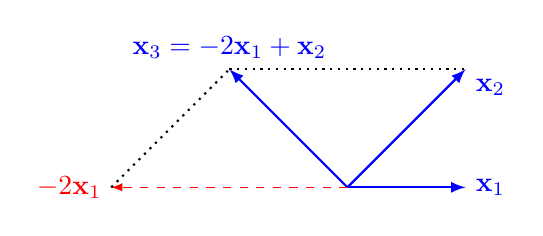
\begin{tikzpicture}[scale=1.5]
  \draw[thick, blue, -latex] (0,0) -- (1, 0) node[right]{$\mathbf{x}_1$};
  \draw[thick, blue, -latex] (0,0) -- (1, 1) node[below right]{$\mathbf{x}_2$};
  \draw[thick, blue, -latex] (0,0) -- (-1, 1) node[above]{$\mathbf{x}_3 = -2\mathbf{x}_1 + \mathbf{x}_2$};
  \draw[dashed, red, -latex] (0,0) -- (-2, 0) node[left]{$-2\mathbf{x}_1$};
  \draw[dotted, thick, black] (-2,0) -- (-1, 1);
  \draw[dotted, thick, black] (-1,1) -- (1, 1);
\end{tikzpicture}
\end{center}
\noindent \textbf{Independence-Dimension inequality}: What is the maximum possible size of a linearly independent collection?
\begin{center}\textit{A linearly independent collection of n-vectors can at most have n vectors.}\end{center}
\end{small}
\end{frame}


\begin{frame}[t]{Basis}
How many vectors can we choose from the following vectors before the set becomes linearly dependent?

\begin{center}
\begin{center}
\tdplotsetmaincoords{70}{110}
\begin{tikzpicture}[scale=3,tdplot_main_coords]
    \def\x{.75}
    \filldraw[draw=white, fill=blue!20] (\x, 0, \x)-- (\x, 0, {-1*\x})-- ({-1*\x}, 0, {-1*\x})-- ({-1*\x}, 0, \x)-- cycle;
    \draw[thick,-latex] (0,0,0) -- (1.5,0,0) node[anchor=north east]{$x$};
    \draw[thick,-latex] (0,0,0) -- (0,1,0) node[anchor=north west]{$y$};
    \draw[thick,-latex] (0,0,0) -- (0,0,1) node[anchor=south]{$z$};
    \draw[thin,dashed] (0,0,0) -- (-0.75,0,0);
    \draw[thin,dashed] (0,0,0) -- (0,-0.5,0);
    \draw[thin,dashed] (0,0,0) -- (0,0,-0.5);
    \draw[thick, red, -] (-1,-1,0) -- (1,1,0);
\end{tikzpicture}
\end{center}
\end{center}

\end{frame}


\begin{frame}[t]{Basis}
\begin{itemize}
  \item A linearly independent set of $n$-vectors from $\mathbb{R}^n$, of size $n$, is called a \textit{basis} for $\mathbb{R}^n$.

  \item Any $n$-vector frtom $\mathbb$ can be represented as a \textit{unique} linear combination of the elements of the basis.
  
  \item Consider the basis $\left\{\mathbf{x}_i\right\}_{i=1}^{n}$, $\mathbf{x}_i \in \mathbb{R}^n$. Any vector $\mathbf{y} \in \mathbb{R}^n$ can be represented as a linear combination of $\mathbf{x}_i$s, $\mathbf{y} = \sum_{i=1}^n \alpha_i\mathbf{x}_i$. This is called the \textit{expansion of} $\mathbf{y}$ in the $\left\{\mathbf{x}_i\right\}_{i=1}^n$ basis.
\end{itemize}
\end{frame}


\begin{frame}[t]{Basis}
\begin{itemize}
  \item The numbers $\alpha_i$ are called the \textit{coefficients} of the expansion of $\mathbf{y}$ in the $\left\{\mathbf{x}_i\right\}_{i=1}^n$ basis.
  
  \item \textbf{Orthogonal vectors}: A set of vectors $\left\{\mathbf{x}_i\right\}_{i=1}^n$ is \textit{(mutually) orthogonal} if $\mathbf{x}_i \perp \mathbf{x}_j$ for all $i, j \in \left\{1, 2, 3, \ldots n\right\}$ and $i \neq j$.
  
  \item This set is called \textbf{orthonormal} if its elements are all of unit length $\left\Vert \mathbf{x}_i \right\Vert_2 = 1$ for all $i \in \left\{1, 2, 3, \ldots n\right\}$.
\end{itemize}
\[ \mathbf{x}_i^T\mathbf{x}_j = \begin{cases} 
      0 & i \neq j \\
      1 & i = j 
   \end{cases}
\]
\end{frame}


\begin{frame}[t]{Representing a Vector in an Orthonormal Basis}
\begin{itemize}
\item An orthonormal collection of vectors is linearly independent.
\item Consider an orthonormal basis $\left\{\mathbf{x}_i\right\}_{i=1}^{n}$. The expansion of a vector $\mathbf{y}$ is given by,
\[ \mathbf{y} = \alpha_1\mathbf{x}_1 + \alpha_2\mathbf{x}_2 + \alpha_3\mathbf{x}_3 + \ldots + \alpha_n\mathbf{x}_n \]
\[ \mathbf{x}_i^T\mathbf{y} = \alpha_1\mathbf{x}_i^T\mathbf{x}_1 + \alpha_2\mathbf{x}_i^T\mathbf{x}_2 + \alpha_3\mathbf{x}_i^T\mathbf{x}_3 + \ldots + \alpha_n\mathbf{x}_i^T\mathbf{x}_n = \alpha_i\]
\end{itemize}
\end{frame}

\begin{frame}[t]{Representing a Vector in an Orthonormal Basis}
\begin{itemize}
\item Thus, we can rewrite this as,
\[ \mathbf{y} = \left(\mathbf{y}^T\mathbf{x}_1\right)\mathbf{x}_1 + \left(\mathbf{y}^T\mathbf{x}_2\right)\mathbf{x}_2 + \left(\mathbf{y}^T\mathbf{x}_3\right)\mathbf{x}_3 + \ldots + \left(\mathbf{y}^T\mathbf{x}_n\right)\mathbf{x}_n \]
\end{itemize}
\begin{center}
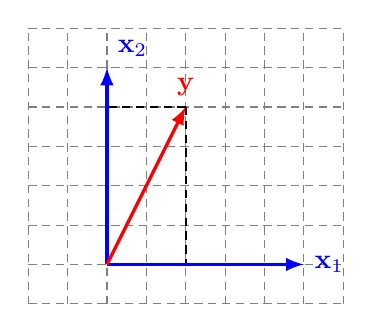
\begin{tikzpicture}[scale=2.5]
  \foreach \x in {-0.4, -0.2, 0, 0.2, 0.4, 0.6, 0.8, 1.0, 1.2}
    \draw[gray, thin, densely dashed] (\x,-0.2)--(\x,1.2);
  \foreach \x in {-0.2, 0, 0.2, 0.4, 0.6, 0.8, 1.0, 1.2}
    \draw[gray, thin, densely dashed] (-0.4,\x)--(1.2,\x);
  \draw[thick, densely dashed, black] (0.4,0.8) -- (0.4,0);
  \draw[thick, densely dashed, black] (0.4,0.8) -- (0.,0.8);
  \draw[very thick, blue, -latex] (0,0) -- (1,0) node[right]{$\mathbf{x}_1$};
  \draw[very thick, blue, -latex] (0,0) -- (0,1) node[above right]{$\mathbf{x}_2$};
  \draw[very thick, red, -latex] (0,0) -- (0.4,0.8) node[above]{$\mathbf{y}$};
\end{tikzpicture}
\end{center}
\end{frame}


\begin{frame}[t]{Dimension of a Vector Space}
\begin{itemize}
\item There an infinite number of bases for a vector space.
\item There is one thing that is common among all these bases -- the number of bases vectors.
\item This number is a property of the vector space, and represents the ``degrees of freedom'' of the space. This is called the \textbf{dimension} of the vector space.
\end{itemize}
\end{frame}


\begin{frame}[t]{Dimension of a Vector Space}
\begin{itemize}
\item A subspace of dimension $m$ can have at most $m$ independent vectors.
\item Notice that the word ``dimension'' of a vector space is different from the ``dimension'' of a vector.
\item E.g. Vectors from $\mathbb{R}^3$ are three dimensional vectors. But the $yz$-plane in $\mathbb{R}^3$ is a 2 dimensional subspace of $\mathbb{R}^3$.
\end{itemize}
\end{frame}


\begin{frame}[t]{Linear Functions}
\begin{itemize}
\item Let $f$ be a function which maps vectors from $\mathbb{R}^n$ to scalar real numbers. It can be represented as the following,
$$f: \mathbb{R}^n \longrightarrow \mathbb{R}; \,\,\,\, y = f(\mathbf{x}) = f\left(x_1, x_2, x_3, \ldots x_n\right)$$

\item Criteria for $f$ to be a linear function:

$$ \textbf{Superposition}: f\left(\alpha \mathbf{x} + \beta \mathbf{y}\right) = \alpha f\left(\mathbf{x}\right) + \beta f\left(\mathbf{y}\right) $$

where $\alpha, \beta \in \mathbb{R}$ and $\mathbf{x}, \mathbf{y} \in \mathbb{R}^n$.
\end{itemize}
\end{frame}



\begin{frame}[t]{Linear Functions}
\begin{itemize}
\item \textbf{Inner product} is a linear function in one of the arguments. $$f\left(x\right) = \mathbf{w}^T\mathbf{x} = w_1x_1 + w_2x_2 + w_3x_3 + \ldots + w_nx_n$$
\item Any linear function can be represented in the form $f\left(\mathbf{x}\right) = \mathbf{w}^T\mathbf{x}$ with an appropriately chosen $\mathbf{w}$.
\end{itemize}
\end{frame}


\end{document}
% -*- root: ../assignment.tex -*-

\subsection*{Matrices}
\begin{enumerate}[resume]
    \item Elements of the matrix $\mf{C} \in \mb{R}^{m \times n}$ obtained as the product of two matrices $\mf{A} \in \mb{R}^{m \times p}$ and $\mf{B} \in \mb{R}^{p \times n}$ is given by,
    \[ c_{ij} = \sum_{k=1}^{p}a_{ik}b_{kj} \]
    We had discussed four different ways to think of matrix multiplication. By algebraically manipulating the previous equation arrive at these four views (inner product view, column view, row view and outer product view)? 

    \item Given the matrices $\mf{A} = \begin{bmatrix*}[r]
    1 & 2 & 3 & 4\\
    -1 & 3 & -1 & -1\\
    2 & -2 & 0 & 2\\
    1 & 0 & -3 & 0\\
    \end{bmatrix*}$, $\mf{B} = \begin{bmatrix*}[r]
    -1 & 1\\
    0 & 1\\
    -1 & 1\\
    -0 & 1\\
    \end{bmatrix*}$ and $\mf{C} = \begin{bmatrix*}[r]
    1 & 1\\
    0 & 1\\
    \end{bmatrix*}$. Evaluate the following products.

    \begin{enumerate*}
        \item $\mf{AB}$
        \item $\mf{A}^2\mf{B}$
        \item $\mf{C}\mf{B}^T\mf{A}$
        \item $\mf{C}^3$
        \item $\mf{ABC}$
    \end{enumerate*}

    \item \textbf{Computational cost of different operations.} What is computational cost of the following matrix operations? Computational cost refers to the number of arithmetic operations  required to carry out a particular matrix operation. Computational cost is a measure of the efficiency of an algorithm. For example, the consider the operation of vector addition, $\mf{a} + \mf{b}$, where $\mf{a}, \mf{b} \in \mb{R}^n$. This requires $n$ addition/subtraction operations and zero multiplication/division operations.
    \begin{enumerate}
        \item Matrix multiplication: $\mf{AB}$, where $\mf{A}, \mf{B} \in \mb{R}^{n \times n}$
        \item Inner product: $\mf{u}^T\mf{v}$
        \item Gaussian Elimination for $\mf{A}\mf{x} = \mf{b}$ where $\mf{A} \in \mb{R}^{n \times n}$, $\mf{x}, \mf{b} \in \mb{R}^{n}$.
        \item Back substitution
        \item Gauss-Jordan method to obtain the row echelon form: $\mf{A} \longrightarrow \mf{E}$.
        \item Matrix inversion using the Gauss-Jordan method: $\bmx \mf{A} \vert \mf{I} \emx \longrightarrow \bmx \mf{I}\vert\mf{A}^{-1}\emx$
    \end{enumerate} 
    Report the counts for the addition/subtraction and multiplication/division operations separately. 

    \item Prove $\ct{\mf{A}\mf{B}}^T = \mf{B}^T\mf{A}^T$.

    \item Consider the following matrix,
    \[ \mf{A} = \bmx \frac{\sqrt{3}}{2} & -\frac{1}{2}\\\frac{1}{2} & \frac{\sqrt{3}}{2} \emx \bmx 0.1 & 0\\0 & 0.9 \emx \bmx \frac{\sqrt{3}}{2} & \frac{1}{2}\\-\frac{1}{2} & \frac{\sqrt{3}}{2} \emx \]
    Find out the expression for $\mf{A}_n = \mf{A}^n$. What is $\mf{A}_\infty = \lim_{n\to\infty} \mf{A}^n$?

    \item Derive force and displacement relationship for a series of $n+1$ springs (with spring constants $k_i$) connected in a line. There are $n$ nodes, with $f_i$ and $x_i$ representing the force applied and resulting displacement at the $i^{th}$ node. 
    \begin{center}
        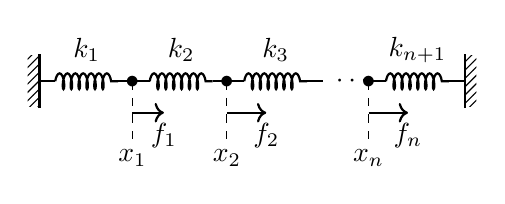
\begin{tikzpicture}
            \fill [pattern = north east lines] (-0.15,-0.325) rectangle (0,0.325);
            \draw[thick] (0,-0.34) -- (0,0.34);

            \draw[thick] (0,0) -- (0.2,0);
            \draw[decoration={aspect=0.3, segment length=1mm, amplitude=1mm, coil,},decorate, thick] (0.2,0) -- (1.0,0);
            \draw[thick] (1.0,0) -- (1.2,0);
            \node[black] at (1.18,-0.02) {$\bullet$};
            \node[black] at (0.6,0.4) {$k_1$};
            \draw[dashed, thin] (1.18,0) -- (1.18,-0.75) node[below]{$x_1$};
            \draw[->,thick] (1.18,-0.4) -- (1.58,-0.4) node[below]{$f_1$};

            
            \draw[thick] (1.2,0) -- (1.4,0);
            \draw[decoration={aspect=0.3, segment length=1mm, amplitude=1mm, coil,},decorate, thick] (1.4,0) -- (2.2,0);
            \draw[thick] (2.2,0) -- (2.4,0);
            \node[black] at (2.38,-0.02) {$\bullet$};
            \node[black] at (1.8,0.4) {$k_2$};
            \draw[dashed, thin] (2.38,0) -- (2.38,-0.75) node[below]{$x_2$};
            \draw[->,thick] (2.38,-0.4) -- (2.88,-0.4) node[below]{$f_2$};
            
            \draw[thick] (2.4,0) -- (2.6,0);
            \draw[decoration={aspect=0.3, segment length=1mm, amplitude=1mm, coil,},decorate, thick] (2.6,0) -- (3.4,0);
            \draw[thick] (3.4,0) -- (3.6,0);
            \node[black] at (3.0,0.4) {$k_3$};

            \node[black] at (4.0, 0) {$\cdots$};

            \draw[thick] (4.2,0) -- (4.4,0);
            \draw[decoration={aspect=0.3, segment length=1mm, amplitude=1mm, coil,},decorate, thick] (4.4,0) -- (5.2,0);
            \draw[thick] (5.2,0) -- (5.4,0);
            \node[black] at (4.18,-0.02) {$\bullet$};
            \node[black] at (4.8,0.4) {$k_{n+1}$};
            \draw[dashed, thin] (4.18,0) -- (4.18,-0.75) node[below]{$x_n$};
            \draw[->,thick] (4.18,-0.4) -- (4.68,-0.4) node[below]{$f_n$};

            \fill [pattern = north east lines] (5.4,-0.325) rectangle (5.55,0.325);
            \draw[thick] (5.4,-0.34) -- (5.4,0.34);
        \end{tikzpicture}
    \end{center}
    \begin{enumerate}
        \item Represent the relationship in the following form,
        \[ \mf{f} = \mf{Kx}; \,\,\, \mf{f} = \begin{bmatrix}f_1\\ f_2\\ \vdots\\ f_n\end{bmatrix}; \,\,\, \mf{x} = \begin{bmatrix}x_1 \\ x_2 \\ \vdots \\ x_n\end{bmatrix}\]
        \item What kind of a pattern does $\mf{K}$ have?
        \item Consider a specific case where $n = 4$ and $k = 1.5 N.m^{-1}$. What should be forces applied at the four nodes in order to displace the spring $\mf{x} = \begin{bmatrix*} 0.5 \\ -0.5 \\ 0 \\ 0 \end{bmatrix*}m$. 
    \end{enumerate}

    \item Prove that a matrix $\mf{M} \in \mathbb{R}^{n \times n}$ can always be written as a sum a symmetric matrix $\mf{S}$ and a skew-symmetric matrix $\mf{A}$.
    \[ \mf{M} = \mf{S} + \mf{A}, \,\,\, \mf{S}^T = \mf{S} \, \text{ and } \, \mf{A}^T = -\mf{A} \]

    Does this property also hold for a complex matrix $\mf{M} \in \mb{C}^{n \times n}$?
    \item The trace of a matrix $\mf{A} \in \mb{R}^{n \times n}$ is defined as, $trace\left(\mf{A}\right) = \sum_{i=1}^{n}a_{ii}$. Prove the following,
    \begin{enumerate}
        \item $trace\left(\mf{A}\right)$ is a linear function of $\mf{A}$.
        \item $trace\left(\mf{AB}\right) = trace\left(\mf{BA}\right)$
        \item $trace\left(\mf{A}^T\mf{A}\right) = 0 \implies \mf{A} = 0$
    \end{enumerate}

    \item Prove that the rank of an outer product $\mf{x}\mf{y}^T$ is 1, where $\mf{x},\mf{y} \in \mb{R}^n$ and $\mf{x}, \mf{y} \neq \mf{0}$.

    \item Is there a relationship between the space of solutions to the following two equations? 
    \[ \mf{y}^T\mf{A} = \mf{c}^T \,\,\,\, \text{ and } \,\,\,\,\, \mf{A}\mf{x} = \mf{b} \]
    If so, how are they related?
    
    \item Consider an upper triangular and lower triangular matrices $\mf{U}$ and $\mf{L}$, respectively. 
    \begin{enumerate}
        \item Is the product of two upper triangular matrices $\mf{U}_1\mf{U}_2$ upper triangular?
        \item Is the product of two lower triangular matrices $\mf{L}_1\mf{L}_2$ upper triangular?
        \item What is the $trace\lp \mf{L}\mf{U} \rp$?
    \end{enumerate}

    \item Consider the following electrical circuit with rectangular grid of resistors $R$. The input to this grid is a set of current injected at the top node as shown in the figure, such that $\sum_{k=1}^5i_k = 0$.
    \vspace{-0.25cm}
    \begin{center}
    \begin{circuitikz}[scale=0.9]
        \draw (2,0) to[R,*-*] (0,0)
        to[R,*-*] (0,2) to[R,*-*] (0,4) to[R,*-*] (2,4)
        to[R,*-*] (2,2) to[R,*-*] (2,0) to[R,*-*] (4,0)
        to[R,*-*] (4,2) to[R,*-*] (4,4) to[R,*-*] (6,4)
        to[R,*-*] (6,2) to[R,*-*] (6,0) to[R,*-*] (8,0)
        to[R,*-*] (8,2) to[R,*-*] (8,4) to[R,*-*] (6,4);

        \draw (0,2) to[R,*-*] (2,2);
        \draw (2,4) to[R,*-*] (4,4);
        \draw (2,2) to[R,*-*] (4,2);
        \draw (4,2) to[R,*-*] (6,2);
        \draw (4,0) to[R,*-*] (6,0);
        \draw (6,2) to[R,*-*] (8,2);

        \draw (0,5) node[above]{$i_1$} to[short, o-] (0,4);
        \draw (2,5) node[above]{$i_2$} to[short, o-] (2,4);
        \draw (4,5) node[above]{$i_3$} to[short, o-] (4,4);
        \draw (6,5) node[above]{$i_4$} to[short, o-] (6,4);
        \draw (8,5) node[above]{$i_5$} to[short, o-] (8,4);
     \end{circuitikz}
     \end{center}

     Express the relationship between the voltages at the different nodes (represented by $\bullet$ in the figure) and the net current flowing in/out of the node in the following form, $\mf{G}\mf{v} = \mf{i}$. Where, $\mf{G}$ is the conductance matrix, $\mf{v}$ is the vector of node voltages, and $\mf{i}$ is the vector representing the net current flow in/out of the different node.

    \item Consider the following system.
    \[\begin{bmatrix*}[r]
    1 & 5 & 1 & 2\\
    2 & -1 & 0 & 2\\
    4 & 0 & 1 & 1\\
    1 & 1 & 0 & 1\\
    \end{bmatrix*}\mf{x}_i = b_i \]
    Solve the above equation using $LU$ factorization for the following $\mf{b}_i$s.
    \[ \mf{b}_1 = \begin{bmatrix*}[r]
    1\\ 0\\ 0\\ 0\\
    \end{bmatrix*}, \,\,\,
    \mf{b}_2 = \begin{bmatrix*}[r]
    0\\ 1\\ 0\\ 0\\
    \end{bmatrix*}, \,\,\,
    \mf{b}_3 = \begin{bmatrix*}[r]
    0\\ 0\\ 1\\ 0\\
    \end{bmatrix*}, \,\,\,
    \mf{b}_4 = \begin{bmatrix*}[r]
    0\\ 0\\ 0\\ 1\\
    \end{bmatrix*}\]

    Construct a matrix $\mf{X}$ using the four solutions $\mf{x}_1, \mf{x}_2, \mf{x}_3$ and $\mf{x}_4$ as its columns.
    \[ \mf{X} = \begin{bmatrix*}\mf{x}_1 & \mf{x}_2 & \mf{x}_3 & \mf{x}_4\end{bmatrix*} \]
    Find out $\mf{XA}$ and $\mf{AX}$,. Based on this what can you say about $\mf{X}$?

    \item How many different reduced row echelon forms can a matrix $\mf{A} \in \mb{R}^{4 \times 5}$ have? Hint: \emph{Think in terms of basic and non-basic columns.}

    \item Consider the system of equation, $\mf{Ax} = \mf{b}$, such that a matrix $\mf{A} \in \mb{R}^{m \times n}$, $\mf{x}, \mf{b} \in \mb{R}^n$. Are the following statements true? Explain your answer.
    \begin{enumerate}
        \item $rank\,\mf{A} \leq \min \lp m, n \rp$
        \item The system is consistent if $\,rank\,\mf{A} = m$.
        \item The system has a unique solution if $\,rank\,\mf{A} = n$.
    \end{enumerate}

    \item Consider a linear function $f: V \to W$, where $V \subset \mb{R}^n$ and $W \subset \mb{R}^m$. If $V$ is a subspace of $\mb{R}^n$ then prove that $W$ is a subspace of $\mb{R}^m$.   

    \item For a $n \times n$ square matrix $\mf{A}$, prove that if $\mf{A}\mf{X} = \mf{I}$, then $\mf{X}\mf{A} = \mf{I}$ and $\mf{X} = \mf{A}^{-1}$.

    \item If two systems of linear equations are consistent, with augmented matices $\left[ \mf{A} | \mf{b}\right]$ and $\left[ \mf{A} | \mf{c}\right]$. Is $\left[ \mf{A} | \mf{b} + \mf{c}\right]$ consistent?

    \item Prove the following for the non-singular square matrices $\mf{A}$ and $\mf{B}$:
    \begin{enumerate}
        \item $\mf{A}\mf{B}$ is non-singular.
        \item $\ct{\mf{A}^{-1}}^{-1} = \mf{A}$.
        \item $\ct{\mf{A}\mf{B}}^{-1} = \mf{B}^{-1}\mf{A}^{-1}$
        \item $\ct{\mf{A}^T}^{-1} = \ct{\mf{A}^{-1}}^T$
    \end{enumerate}

    \item If a matrix $\mf{A}$ has LU decomposition, such that $\mf{A} = \mf{LU}$. Demonstrate that it also has a LDU decomposition $\mf{A} = \mf{LD}\hat{\mf{U}}$, where $\mf{D}$ is a diagonal matrix, and $\hat{\mf{U}}$ is upper triangular. What happens to the LU and LDU decompositions when a matrix $\mf{A} = \mf{A}^T$?

    \item Write down a basis for the four fundamental subspaces of the following matrix,
    \[ \mf{A} = \begin{bmatrix*}[r]
    1 & 2 & -3 & 4 & -1 & 0 \\
    4 & 8 & 12 & -8 & 2 & 1 \\
    2 & 3 & 2 & 1 & -2 & 0 \\
    -3 & -1 & 1 & -4 & 0 & -1 \\
    1 & -2 & -1 & 0 & 0 & 0 \\
    \end{bmatrix*} \]
    
    \item Consider a matrix $\mf{A} = \begin{bmatrix*}[r] 1 & 4 & 5\\ 4 & 118 & 26\\3 & 16 & 30\end{bmatrix*}$.
    \begin{enumerate}
        \item Apply Gaussian elimination to simply this matrix into an upper-triangular matrix $\mf{U}$.
        \item What is the corresponding upper-triangular matrix $\tilde{\mf{U}}$ obtained by applying Gaussian elimination to $\mf{A}^T$? 
        \item Could you have arrived at $\tilde{\mf{U}}$ without having to repeat the Gaussian elimination process on $\mf{A}^T$?
        \item Write down the LDU decompositions of $\mf{A}$ and $\mf{A}^T$.
    \end{enumerate} 

    \item Derive the inverse of the matrix $\mf{A} = \begin{bmatrix}a & b\\c & d\end{bmatrix}$.
    
    \item Consider the following upper-triangular matrix, 
    $$U = \begin{bmatrix}
    u_{11} & u_{12} & u_{13} & \cdots & u_{1n}\\
    0 & u_{22} & u_{23} & \cdots & u_{2n}\\
    0 & 0 & u_{33} & \cdots & u_{3n}\\
    \vdots & \vdots & \vdots & \ddots & \vdots\\
    0 & 0 & 0 & \cdots & u_{nn}\\\end{bmatrix}$$
    where, $u_{ii} \neq 0, \,\,\, 1 \leq i \leq n$. Do the columns of this matrix form a linearly independent set? Explain your answer.

    \item Verify that $\mf{A}$ and $\mf{B}$ are inverses of each other,
    \begin{enumerate}
        \item $\mf{A} = \mf{I} - \mf{u}\mf{v}^T$ and $\mf{B} = \mf{I} + \mf{u}\mf{v}^T / \lp 1 - \mf{v}^T\mf{u} \rp$
        \item $\mf{A} = \mf{C} - \mf{u}\mf{v}^T$ and $\mf{B} = \mf{C}^{-1} + \mf{C}^{-1}\mf{u}\mf{v}^T\mf{C}^{-1} / \lp 1 - \mf{v}^T\mf{C}^{-1}\mf{u} \rp$
        \item $\mf{A} = \mf{I} - \mf{U}\mf{V}$ and $\mf{B} = \mf{I}_{n} + \mf{U}\lp \mf{I}_m - \mf{V}\mf{U}\rp^{-1}\mf{V}$
        \item $\mf{A} = \mf{C} - \mf{U}\mf{D}^{-1}\mf{V}$ and $\mf{B} = \mf{A}^{-1} + \mf{A}^{-1}\mf{U}\lp \mf{D} - \mf{V}\mf{A}^{-1}\mf{U}\rp^{-1}\mf{V}\mf{A}^{-1}$
    \end{enumerate}
    where, $\mf{A}, \mf{B} \in \mb{R}^{n \times n}$, $\mf{u}, \mf{v} \in \mb{R}^n$, $\mf{U} \in \mb{R}^{n \times m}$, $\mf{V} \in \mb{R}^{m \times n}$ and $\mf{D} \in \mb{R}^{m \times m}$.

    \item Consider the matrices $\mf{A} \in \mb{R}^{m \times m}$, $\mf{B} \in \mb{R}^{n \times n}$ and $\mf{C} \in \mb{R}^{m \times n}$. Verify the following,
    \begin{enumerate}
        \item $\bmx \mf{A} & \mf{0} \\ \mf{0} & \mf{B}\emx^{-1} = \bmx \mf{A}^{-1} & \mf{0} \\ \mf{0} & \mf{B}^{-1}\emx$
    \end{enumerate}
    
    \item Gaussian elimination does not change the solution of a system $\mf{A}\mf{x} = \mf{b}$. Explain why the three row operations do not affect the solution of the system. Instead of row operations, what if we performed column operations. Will the solution of the system $\mf{Ax} = \mf{b}$ still remain unchanged? If the solution is affected, how is it affected by the following operations?
    \begin{enumerate}
        \item Columns $\mf{a}_i$ and $\mf{a}_j$ of $\mf{A}$ are interchanged.
        \item Column $\mf{a}_i$ is replaced by $\alpha\mf{a}_i$.
        \item Columns $\mf{a}_i$ is replace by $\mf{a}_i + \beta\mf{a}_j$.
    \end{enumerate}

    \item \textbf{Two point boundary problem.} $\mf{A}\mf{x} = \mf{b}$ is often encountered in many practical applications. One such application is the numerical solution of differential equations of the following form,
    \[ \sum_{i=0}^M a_{i}\ct{x}y^{\ct{i}}\ct{x} = f\ct{x} \]
    where, $x \in \dt{a, b}$ and $y\ct{a} = \alpha, y\ct{b} = \beta$. 

    Numerical methods are often employed for obtaining an approximate estimate of $y\ct{x}$ at discrete points in the interval $\dt{a,b}$. The interval is divided into subintervals of width $\Delta x$. The derivate of $y\ct{x}$ at the different nodes (points between two subintervals) can be approximated as the following,
    \begin{align}
    y'\ct{x_i} &= \frac{y\ct{x_i + \Delta x} - y\ct{x_i - \Delta x}}{\Delta x}\nonumber\\
    y''\ct{x_i} &= \frac{y\ct{x_i + \Delta x} + 2y\ct{x_i} - y\ct{x_i - \Delta x}}{\Delta x^2} \nonumber
    \end{align}
    where, $x_i = a + i\Delta x, \,\, 0 \leq i \leq N+1$, and $b - a = \ct{N+1} \Delta x$. Addition and subtracting the above two equations and neglecting terms involving higher orders of $\Delta x$, we get the following approximations for the derivatives of $y\ct{x}$ at $x_i$.

    Replacing the derivatives of $y\ct{x}$ by the above approximations and evaluating the equation at the different nodes $x_i$s, we arrive a set of $N$ linear equations with $N$ unknowns $y\ct{x_1}, y\ct{x_2}, \ldots y\ct{x_N}$. 

    Using this approach, compute an approximate solution for $y\ct{x}$ for the following differential equations over the interval $x \in \dt{0, 1}$. 
    \begin{enumerate}
         \item $y''\ct{x} = -x$
         \item $y''\ct{x} + y'\ct{x} = x$
    \end{enumerate}
    Solve these equations for different values of $\Delta x$, and compare the resulting approximate solution for $y\ct{x}$ with the exact solution.   Present your results as a plot the solution $y\ct{x_i}$ versus $x_i$.

    Comment on the dependence of the solution $\ct{x}$ on $\Delta x$. What is the best value for $\Delta x$ to use in solving these equations?

    \item \label{matrices:uncertain} \textbf{Ill-conditioned systems.} A system $\mf{A}\mf{x} = \mf{b}$ is said to be ill-conditioned when small changes in the components of $\mf{A}$ or $\mf{b}$ can produce large changes in the solution $\mf{x}$. Consider the following system,
    \begin{align}
    x - y &= 100 \nonumber \\
    10 + \ct{9 + \Delta}y &= 0 \nonumber
    \end{align}
    Find the solutions of the system for different values of $\Delta = -2, -1, 0, 1, 2$. How do the solutions change with $\Delta$. Now consider the following system,
    \begin{align}
    x - y &= 100 \nonumber \\
    10 - \ct{9 + \Delta}y &= 0 \nonumber
    \end{align}
    The second system is an example of an ill-conditioned system. What can you say about the geometries of these two systems?

    \item \textbf{Connectivity matrices.} Another common application of matrices is in graph theory. A graph is a set of vertices or nodes connected by edges, as show in the following figure. $A$-$F$ are the nodes of the graph, and the lines with the arrows are the edges that convey information about the connections or relationships between the nodes.
    \begin{center}
        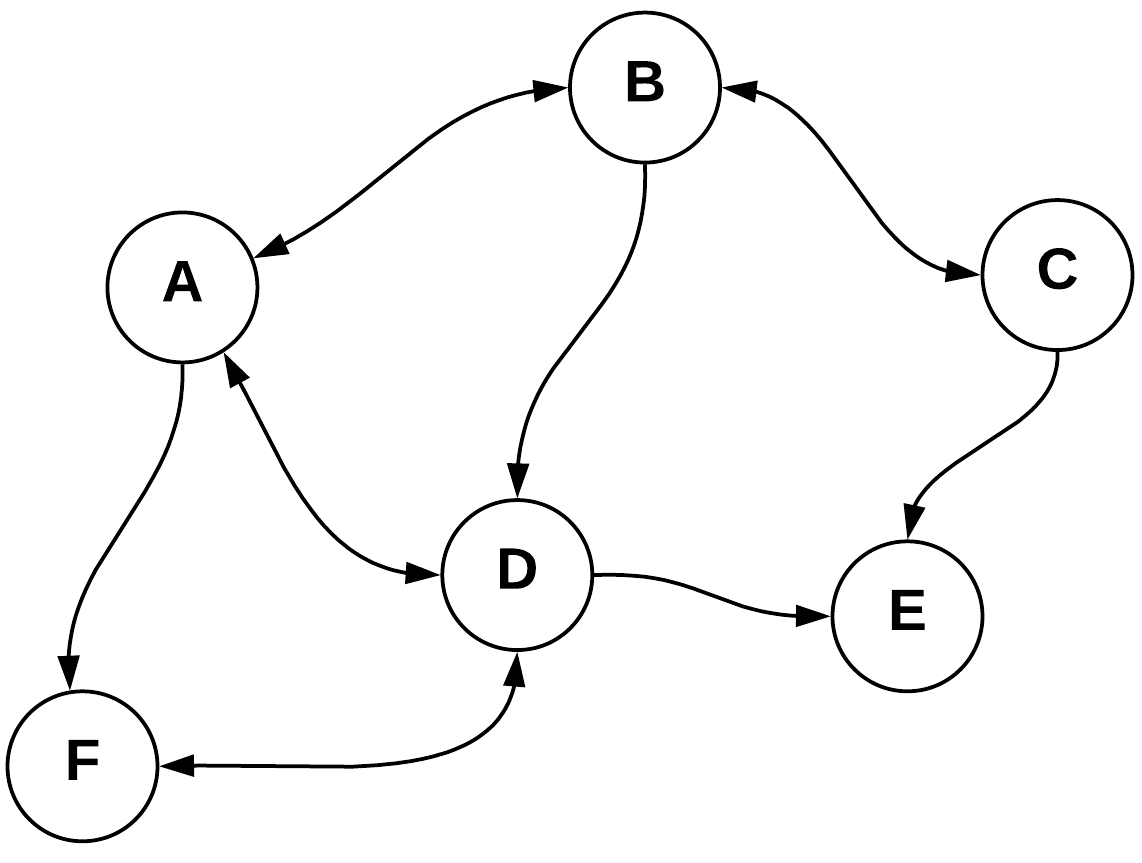
\includegraphics[width=0.5\columnwidth]{sections/figs/graph.png}
    \end{center}
    The above graph can be thought as a representation of different places in a city (represented by the nodes), and the lines with the arrows represent the roads connecting these different places. A line with two arrows allow two-way traffic, while line with single arrow only allow one way traffic. The connectivity between the different places can be summarized though the connectivity matrix $\mf{C} \in \mb{R}^{n \times n}$, where $n$ is the number of nodes in the graph. The elements of this connectivity matrix  represents whether or not there is a direct path between two places.
    \[ 
    c_{ij} = \begin{cases}
        1 & \text{there is a direct road between places } i \, \& \,j. \\
        0 & \text{otherwise.}
    \end{cases}
    \]
    The diagonal element of $\mf{C}$ are zero, $c_{ii} = 0$.

    Write down the connectivity matrix $\mf{C}$ for the graph shown above. How can we use the matrix $\mf{C}$ to answer the following questions? Explain exact matrix operation you would perform to answer these questions (Hint: Consider higher power of $\mf{C}$).
    \begin{enumerate}
        \item Is there a path between two places $i$ and $j$ that goes via one other place? For example, we can go from $A$ to $D$ via $B$.
        \item How many paths are there between places $i$ and $j$ that goes via three other places?
    \end{enumerate}
\end{enumerate}
% -*- root: ../assignment.tex -*-
\subsection*{Orthogonality}
\begin{enumerate}[resume]
    \item Consider an orthonormal set of vectors $V = \left\{ \mf{v}_1, \mf{v}_2, \ldots \mf{v}_r\right\},\,\,\, \mf{v}_i \in \mb{R}^n\,\,\,\forall i \in \left\{1, 2, \ldots r\right\}$. If there is a vector $\mf{w} \in \mb{R}^n$ such that $\mf{v}_i^T\mf{w} = 0\,\,\,\forall i \in \left\{1, 2, \ldots r\right\}$. Prove that $\mf{w} \notin span\left(V\right)$.
    
    \item Consider the following set of vectors in $\mb{R}^4$.
    \[ V = \left\{
    \bmx
    1\\-2\\0\\3
    \emx,
    \bmx
    1\\1\\1\\1
    \emx,
    \bmx
    2\\-1\\1\\4
    \emx
    \right\} \]
    Find the set of all vectors that are orthogonal to $V$?

    \item For a matrix $\mf{A} \in \mb{R}^{m \times n}$, prove that $C\lp\mf{A}\rp \perp N\lp\mf{A}^T\rp$ and $C\lp\mf{A}^T\rp \perp N\lp\mf{A}\rp$.

    \item If the columns of a matrix $\mf{A} \in \mb{R}^{n \times n}$ are orthonormal, prove that $\mf{A}^{-1} = \mf{A}^T$. What is $\mf{A}^T\mf{A}$ when $\mf{A}$ is rectangular $\left(\mf{A} \in \mb{R}^{m \times n}\right)$ with orthonormal columns?

    \item What will happen when the Gram-Schmidt procedure is applied to: (a) orthonormal set of vectors; and (b) orthogonal set of vectors? If the set of vectors are columns of a matrix $\mf{A}$, then what are the corresponding $\mf{Q}$ and $\mf{R}$ matrices for the orthonormal and orthogonal cases?

    \item Consider the linear map, $\mf{y} = \mf{Ax}$, such that $\mf{x}, \mf{y} \in \mb{R}^n$ and $\mf{A} \in \mb{R}^{n \times n}$. Let us assume that $\mf{A}$ is full rank. What conditions must $\mf{A}$ satisfy for the following statements to be true,
    \begin{enumerate}
        \item $\left\lVert \mf{y}\right\rVert_2 = \left\lVert \mf{x}\right\rVert_2$, for all $\mf{x}, \mf{y}$ such that $\mf{y} = \mf{Ax}$.
        \item $\mf{y}_1^T\mf{y}_2 = \mf{x}_1^T\mf{x}_2$, for all $\mf{x}_1, \mf{x}_2, \mf{y}_1, \mf{y}_2$ such that $\mf{y}_1 = \mf{A}\mf{x}_1$ and $\mf{y}_2 = \mf{A}\mf{x}_2$. 
    \end{enumerate}
    \vspace{-0.1cm}
    \begin{color}{black!60}\small{\textbf{Note}: A linear map $\mf{A}$ with the aforementioned properties preserves lengths and angle between vectors. Such maps are encountered in rigid body mechanics.}
    \end{color}

    \item Prove that the rank of an orthogonal projection matrix $\mf{P}_{S} = \mf{UU}^T$ onto a subspace $\mc{S}$ is equal to the $\text{dim } \mc{S}$, where the columns of $\mf{U}$ form an orthonormal basis of $\mc{S}$.

    \item If the columns of $\mf{A} \in \mb{R}^{m \times n}$ represent a basis for the subspace $\mc{S} \subset \mb{R}^m$. Find the orthogonal projection matrix $\mf{P}_\mc{S}$ onto the subspace $\mc{S}$. Hint: Gram-Schmidt orthogonalization.

    \item Consider two orthogornal matrices $\mf{Q}_1$ and $\mf{Q}_2$. Is the $\mf{Q}_2^T\mf{Q}_1$ an orthogonal matrix? If yes, prove that it is so, else provide a counter-example showing $\mf{Q}_2^T\mf{Q}_1$ is not orthogonal.

    \item Let $\mf{P}_\mc{S}$ represent an orthogonal projection matrix onto to the subspace $\mc{S} \subset \mb{R}^n$. What can you say about the rank of the matrix $\mf{P}_\mc{S}$? Explain how you can obtain an orthonormal basis for $\mc{S}$ from $\mf{P}_\mc{S}$.

    \item Consider a 1 dimensional subspace spanned by the vector $\mf{u} \in \mb{R}^n$. What kind of a geometric operation does the matrix $\mf{I} - 2\frac{\mf{u}\mf{u}^T}{\mf{u}^T\mf{u}}$ represent?

    \item Prove that when a triangular matrix is orthogonal, it is diagonal.

    \item If an orthogonal matrix $\mf{Q} \in \mb{R}^{n \times n}$ is to be partitioned such that, $\mf{Q} = \bmx \mf{Q}_1 & \mf{Q}_2\emx$, then prove that $C\lp\mf{Q}_1\rp \perp C\lp\mf{Q}_2\rp$.

    \item Find an orthonormal basis for the subspace spanned by $\lc \bmx1\\-1\\2\emx, \bmx-1\\-1\\-1\emx, \bmx1\\-3\\3\emx \rc$.

\end{enumerate}

% -*- root: ../assignment.tex -*-
\subsection*{Matrix Inverses}
\begin{enumerate}[resume]
    \item Consider the following bases for $\mb{R}^3$.
    \[ A^S = \lc \frac{1}{\sqrt{3}}\bmx1 \\ 1 \\ 1\emx, \frac{1}{\sqrt{6}}\bmx-1 \\ 2 \\ -1\emx, \frac{1}{\sqrt{2}}\bmx1 \\ 0 \\ -1\emx \rc \]
    \[ B^A = \lc \frac{1}{\sqrt{5}}\bmx2 \\ 1 \\ 0\emx, \frac{1}{\sqrt{5}}\bmx-1 \\ 2 \\ 0\emx, \bmx0 \\ 0 \\ 1\emx \rc \]

    Where,  $X^Y$ is the basis $X$ represented in another basis $Y$; $S$ stands for the standard basis. Let $\mf{b}_X$ stand for the representation of vector in $\mb{R}^3$ in the basis $X$. 
    \begin{enumerate}
        \item Consider a vector $\mf{b}_S = \bmx-1\\0\\2\emx$ represented in the standard basis. What is the representation of $\mf{b}_S$ in the other four basis $A$, and $B$?

        \item Consider a vector $\mf{d}_B = \bmx-1\\-1\\0\emx$ represented in the basis $B$. What is the representation of this vector in the standard basis?
    \end{enumerate}


    \item When does the following diagnoal matrix have an inverse?
    \[ \mf{D} = \begin{bmatrix*}
    d_1 & 0 & 0 & \ldots & 0\\
    0 & d_2 & 0 & \ldots & 0\\
    0 & 0 & d_3 & \ldots & 0\\
    \vdots & \vdots & \vdots & \ddots & \vdots\\
    0 & 0 & 0 & \ldots & d_n\\\end{bmatrix*} \]
    Write down an expression for $D^{-1}$.
    
    \item Prove that the inverse of a non-singular upper-triangular matrix is upper-triangular. Using this show that for a lower triangular matrix it is lower-triangular.

    \item Consider a $2 \times 2$ block matrix, $\mf{A} = \bmx \mf{B} & \mf{C}\\\mf{D} & \mf{E}\emx$, where $\mf{A} \in \mb{R}^{m \times m}$. Find an expression for the inverse $\mf{A}^{-1}$ interms of the block components and their inverses (if they exist) of $\mf{A}$. Hint: Consider $\mf{A}^{-1} = \bmx \mf{P} & \mf{Q}\\ \mf{R} & \mf{S}\emx$, and solve $\mf{A}\mf{A}^{-1} = \mf{I}$.

    \item Express the inverse of the following matrix in terms of $\mf{A}$ and $\mf{b}$. 
    \[ \mf{H} = \begin{bmatrix*}
    \mf{A} & \mf{b}\\
    \mathbf{0} & 1\\
    \end{bmatrix*} \in \mathbb{R}^{\left(n+1\right) \times \left(n+1\right)}
    \]
    where, $\mf{A} \in \mathbb{R}^{n \times n}$ and $\mf{b} \in \mathbb{R}^n$. 

    \item Consider a matrix $\mf{A} \in \mathbb{R}^{m \times n}$ with linearly independent columns. Prove that the Gram matrix $\mf{A}^T\mf{A}$ is invertible.
    
    \item Find all possible left/right inverses for the following matrices, if they exist.
    \begin{enumerate}
        \item $\mf{A} = \bmx 1 & 1 & 1 & 1\\ -1 & -2 & -3 & -4\emx$
        \item $\mf{A} = \bmx 1 & -1 & 0 & 0 & -2\\ 0 & 0 & 1 & 0 & 3\\0 & 0 & 0 & 1 & -1\emx$
        \item $\mf{A} = \bmx 1 & 2\\-1 & 0\\-3 & 4\emx$
        \item $\mf{A} = \bmx 1 & 1 & 1 & 1 & 1\\
        1 & 2 & 2 & 2 & 2\\
        1 & 2 & 3 & 3 & 3\\
        1 & 2 & 3 & 4 & 5\\
        1 & 2 & 3 & 4 & 5
        \emx$
    \end{enumerate}
    
    For each of these matrices find the corresponding pseudo-inverse $\mf{A}^{\dagger}$, and verify that the pseudo-inverse has the minimum squared sum of its components.

    \item Prove that the inverse of a non-singular symmetric matrix is symmetric.

    \item Consider the scalar equation, $ax = ay$. Here we can cancel $a$ from the equation when $a \neq 0$. When can we carry out similar cancellations for matrcies?
    \begin{enumerate}
        \item $\mf{A}\mf{X} = \mf{A}\mf{Y}$. Prove that here $\mf{X}=\mf{Y}$ only when $\mf{A}$ is left invertible.
        \item $\mf{X}\mf{A} = \mf{Y}\mf{A}$. Prove that here $\mf{X}=\mf{Y}$ only when $\mf{A}$ is right invertible.
    \end{enumerate}

    \item Consider two non-singular matrices $\mf{A}, \mf{B} \in \mb{R}^{n \times n}$. Explain whether or not the following matrices are invertible. If they are, then provide an expression for it inverse.
    \begin{enumerate}
        \item $\mf{C} = \mf{A} + \mf{B}$
        \item $\mf{C} = \bmx \mf{A} & \mf{0}\\\mf{0} & \mf{B}\emx$
        \item $\mf{C} = \bmx \mf{A} & \mf{A} + \mf{B}\\\mf{0} & \mf{B}\emx$
        \item $\mf{C} = \mf{A}\mf{B}\mf{A}$
    \end{enumerate}

    \item Consider the matrices $\mf{A} \in \mb{R}^{m \times l_1}$ and $\mf{B} \in \mb{R}^{l_2 \times m}$. Can you find the requirements for matrices $\mf{A}$ and $\mf{B}$, such that $\mf{A}\mf{X}\mf{B} = \mf{I}$, where $\mf{X} \in \mb{R}^{l_1 \times l_2}$? Assuming those conditions are satisfied,  find an expression for $\mf{X}$?

    \item Consider a matrix $\mf{C} = \mf{A}\mf{B}$, where $\mf{A} \in \mf{R}^{m \times n}$ and $\mf{B} \in \mf{R}^{n \times m}$. Explain why $\mf{C}$ is not invertible when $m > n$. Suppose $m < n$, under what conditions is $\mf{C}$ invertible?

    % \item For a non-singular square matrix $\mf{A}$, prove that $\lp\mf{A}^T\rp^{-1} = \lp\mf{A}^{-1}\rp^T$.

    \item For a square matrix $\mf{A}$ with non-signular $\mf{I} - \mf{A}$, prove that $\mf{A}\lp\mf{I} - \mf{A}\rp^{-1} = \lp\mf{I} - \mf{A}\rp^{-1}\mf{A}$.

    \item Consider the non-singular matrices $\mf{A}$, $\mf{B}$ and $\mf{A} + \mf{B}$. Prove that,
    \[ \mf{A}\lp\mf{A} + \mf{B}\rp^{-1}\mf{B} = \mf{B}\lp\mf{A} + \mf{B}\rp^{-1}\mf{A} = \lp\mf{A}^{-1} + \mf{B}^{-1}\rp^{-1} \]

\end{enumerate}
% \vfill
% -*- root: ../assignment.tex -*-
\subsection*{Eigenvalues and Eigenvectors}
\begin{enumerate}[resume]
    \item Explain why an eigenvector cannot be associated with two eigenvalues.

    \item What are the eigenspaces associated with the diagonal matrix $\mf{D} = \mathrm{diag}\lp d_1, d_2, \ldots d_n\rp$?

    \item If a matrix $\mf{A}$ has zero as one of its eigenvalues, explain why $\mf{A}$ must be singular.

    \item For a matrix $\mf{A}$ with eigenvalues $\lc\lambda_i\rc_{i=1}^{n}$, verify for the following matrices that $\Pi_{i=1}^n\lambda_i = \det \lp\mf{A}\rp$ and $\sum_{i=1}^n \lambda_i = trace\lp\mf{A}\rp$.
    \begin{enumerate}
        \item $\bmx 1 & 1 \\ 2 & 1\emx$
        \item $\bmx 1 & 0 & -1 \\ -1 & 1 & 0 \\ 2 & 1 & 1\emx$
        \item $\bmx 1 & 1 \\ 0 & 1\emx$
        \item $\frac{1}{5}\bmx 1 \\ 0 \\ 2 \emx \bmx 1 & 0 & 2\emx$
    \end{enumerate}

    \item Let $\lc\lambda_i, \mf{v}_i\rc_{i=1}^n$ be the eigenpairs of a matrix $\mf{A}$. Then prove that,
    \begin{enumerate}
        \item $\lc\lambda_i^k, \mf{v}_i\rc_{i=1}^n$ are the eigenpairs of $\mf{A}^k$. 
        \item $\lc p\lp\lambda_i\rp, \mf{v}_i\rc_{i=1}^n$ are the eigenpairs of $p\lp\mf{A}\rp$, where $p\lp \mf{A}\rp = \alpha_0\mf{I} + \alpha_1\mf{A} + \ldots + \alpha_k\mf{A}^k$.
    \end{enumerate}

    \item Prove that if $\lc\lambda_i, \mf{v}_i\rc_{i=1}^n$ are the eigenpairs of a matrix $\mf{A}$, then the eigenpairs of $\mf{A}^k$ are $\lc\lambda_i^k, \mf{v}_i\rc_{i=1}^n$. 

    \item Consider the matrices $\mf{A} = \bmx 1 & 1\\ 0 & 1 \emx$, $\mf{B} = \bmx 2 & 0 \\ 1 & 1\emx$. Are the eigenvalues of $\mf{A}\mf{B}$ equal the eigenvalues of $\mf{B}\mf{A}$?

    \item Consider the matrices $\mf{A}$ and $\mf{B}$. If $\mf{v}$ is an eigenvector $\mf{B}$, underwhat condition will $\mf{v}$ also be the eignevector of $\mf{A}\mf{B}$. Under these conditions, what will be corresponding eigenvalue of $\mf{v}$? How do your answers change in the case of $\mf{BA}$?

    \item Let $\lc \lambda_i, \mf{v}_i\rc_{i=1}^n$ are the eignepairs of a matrix $\mf{A}$. What are the eigenpairs of the folliowing?
    \begin{enumerate}
         \item $2\mf{A}$
         \item $\mf{A} - 2\mf{I}$
         \item $\mf{I} - \mf{A}$
     \end{enumerate}

     \item Let $\mf{A} = \bmx 0.6 & 0.2\\ 0.4 & 0.8\emx$. What is the value of:
     \begin{enumerate*}
         \item $A^2$
         \item $A^{100}$
         \item $A^\infty$
     \end{enumerate*}?

     \item Show that $\mf{u} \in \mb{R}^2$ is an eigenvector of $\mf{A} = \mf{u}\mf{v}^T$. What are the two eigenvalues of $\mf{A}$?

     \item Consider two similar matrices $\mf{A}$ and $\mf{B}$. Prove that the eigenvalues of $\mf{A}$ and $\mf{B}$ are the same. How are the eigenvectors of $\mf{A}$ and $\mf{B}$ related to each of other for a given eigenvalue?

     \item Find the eigenvectors of the following permutation matrix $\mf{A} = \bmx 0 & 1 & 0\\ 1 & 0 & 0 \\ 0 & 0 & 1\emx$.

     \item \textbf{Left eigenvectors}: Consider a matrix $\mf{A}$ with eigenpairs $\lc \lambda_1, \mf{v}_i\rc_{i=1}^n$. The left eigenvectors of the matrix $\mf{A}$ are the vectors that satisfy the equation, $\mf{A}^T\mf{w} = \mu \mf{w}$ (or $\mf{w}^T\mf{A} = \mu \mf{w}^T$), and let $\lc \mu_i, \mf{w}_i\rc_{i=1}^n$ be the left eigenpairs of $\mf{A}$. Show the following,
     \begin{enumerate}
         \item The eigenvalues of both $\mf{A}$ and $\mf{A}^T$ are the same.
         \item $\mf{v}_i^T\mf{w}_j = 0$. The eigenvector $\mf{v}_i$ corresponding to the eigenvalue $\lambda_i$ and the left eigvenvector $\mf{w}_j$ corresponding to the eigenvalue $\lambda_j$ are orthogonal, when $\lambda_i \neq \lambda_j$.
         \item The matrix $A$ can be expressed as a sum of rank-one matrices,
         \[ \mf{A} = \lambda_1\mf{v}_1\mf{w}_1^T + \lambda_2\mf{v}_2\mf{w}_2^T + \ldots + \lambda_n\mf{v}_n\mf{w}_n^T\]
     \end{enumerate}

     \item Prove that $\mf{A}\mf{A}^T$ has real and positive eigenvalues, and that the eigenvectors corresponding to distinct eigenvalues of $\mf{A}\mf{A}^T$ are orthogonal.

     \item If $\lc \lambda_i, \mf{v}_i\rc_{i=1}^n$ are the eigenpairs of a non-singular matrix $\mf{A}$, the prove that $\lc \lambda_i^{-1}, \mf{v}_i\rc_{i=1}^n$ are the eigenpairs of $\mf{A}^{-1}$.

     \item A matrix $\mf{A}$ is called \textit{nilpotent} if $\mf{A}^k = \mf{0}$ for some finite positive integer $k$. Prove that the $trace\lp \mf{A}\rp = 0$ for a nilpotent matrix $\mf{A}$. What are all the eigenvalues of such a matrix?

\end{enumerate}
% \vfill
% -*- root: ../assignment.tex -*-
\subsection*{Positive Definite Matrices and Matrix Norm}
\begin{enumerate}[resume]
    \item Prove that $\mf{A}^T\mf{A}$ is positive semi-definite for any matrix $\mf{A}$. When is $\mf{A}^T\mf{A}$ guaranteed to be positive definite?

    \item If $\mf{A}$ is positive definite, then prove that $\mf{A}^{-1}$ is also positive definite.

    \item Show that a positive definite matrix cannot have a zero or a negative element along its diagonal.

    \item Show that the following statements are true.
        \begin{enumerate}
            \item All positive definite matrices are inverstible.
            \item The only positive definite projection matrix is $\mf{I}$.
        \end{enumerate}

    \item Is the function $f\lp x_1, x_2, x_3\rp = 12 x_1^2 + x_2^2 + 6x_3^2 + x_1x_2 - 2x_2x_3 + 4x_3x_1$ positive definite?

    \item The $LU$ decomposition for symmetric matrices can be written as $\mf{A} = \mf{L}^T\mf{D}\mf{L}$, where $\mf{D}$ is a diagonal matrix, and $\mf{L}$ is lower triangular with $1$ along its main diagonal. When $\mf{A}$ is postive definite, we can write, $\mf{A} = \mf{C}^T\mf{C} = \mf{L}^T\sqrt{\mf{D}}\sqrt{\mf{D}}\mf{L}$. This is the \textit{Cholesky decomposition}. Find $\mf{C}$ for the following,
    \begin{enumerate}
        \item $\bmx 4 & 1\\ 1 & 2\emx$
        \item $\bmx 4 & 1 & 0\\ 1 & 8 & 0\\0 & 0 & 2\emx$
    \end{enumerate}

    \item Prove the following for $\mf{A} \in \mb{R}^{m \times n}$:
    \[ \mf{A} = \bmx \mf{a}_1 & \mf{a}_2 & \ldots & \mf{a}_n\emx = \bmx \tilde{\mf{a}_1^T}\\ \tilde{\mf{a}_1^T} \\ \vdots \\ \tilde{\mf{a}_m^T}\emx \]
    \begin{enumerate}
        \item $\lV\mf{A}\rV_1 = \max_{1 \leq i \leq n} \lV\mf{a}_i\rV_1$
        \item $\lV\mf{A}\rV_\infty = \max_{1 \leq i \leq m} \lV\tilde{\mf{a}}_i\rV_1$
        \item $\lV\mf{A}\rV_2 = \max_{1 \leq i \leq n} \lv \lambda_i \rv$, where $\lambda_i$ are the eigenvalues of $\mf{A}^T\mf{A}$.
        \item $\lV\mf{A}\rV_F = trace\lp \mf{A}^T\mf{A}\rp$
    \end{enumerate}

    \item Prove that the induced norm of a matrix product is bounded: $\lV\mf{A}\mf{B}\rV \leq \lV\mf{A}\rV\lV\mf{B}\rV$.

    \item Verify the following inequalities on vector and matrix norms ($\mf{x} \in \mb{R}^m$ and $\mf{A} \in \mb{R}^{m \times n}$):
    \begin{enumerate}
        \item $\lV\mf{x}\rV_\infty \leq \lV\mf{x}\rV_2$
        \item $\lV\mf{x}\rV_2 \leq \sqrt{m}\lV\mf{x}\rV_\infty$
        \item $\lV\mf{A}\rV_\infty \leq \sqrt{n}\lV\mf{A}\rV_2$
        \item $\lV\mf{A}\rV_2 \leq \sqrt{m}\lV\mf{A}\rV_\infty$
    \end{enumerate}

    \item Find an expression for the induced 2-norm of an outer product, $\mf{A} = \mf{u}\mf{v}^T$, where $\mf{u} \in \mb{R}^m$ and $\mf{v} \in \mb{R}^n$.
\end{enumerate}
% \vfill
\documentclass[9pt]{article}

\usepackage[utf8]{inputenc}
\usepackage{geometry}
\geometry{
    a4paper,
    total={170mm,257mm},
    left=15mm,
    right=15mm,
    top=20mm,
    bottom=20mm,
}
\usepackage{multicol}
\usepackage[font=small,labelfont=bf]{caption}
\setlength{\columnsep}{0.25cm}
\usepackage[inline]{enumitem}
\usepackage{amssymb}
\usepackage{xcolor}
\usepackage{mathtools} 
\setlength{\parindent}{0em}
\setlength{\parsep}{0em}
\usepackage{tikz}
\setlength{\parskip}{0em}
\usetikzlibrary{decorations.pathmorphing,patterns}
\usepackage[american,cuteinductors]{circuitikz}
\usetikzlibrary{shapes,arrows,circuits,calc,babel}
% Definition of blocks:
\tikzset{%
  block/.style    = {draw, thick, rectangle, minimum height = 3em,
    minimum width = 3em},
  sum/.style      = {draw, circle, node distance = 2cm}, % Adder
  input/.style    = {coordinate}, % Input
  output/.style   = {coordinate} % Output
}
% Defining string as labels of certain blocks.
\newcommand{\suma}{\Large$+$}
\newcommand{\inte}{$\displaystyle \int$}
\newcommand{\derv}{\huge$\frac{d}{dt}$}

\def\mf{\ensuremath\mathbf}
\def\mb{\ensuremath\mathbb}
\def\mc{\ensuremath\mathcal}
\def\lp{\ensuremath\left(}
\def\rp{\ensuremath\right)}
\def\lv{\ensuremath\left\lvert}
\def\rv{\ensuremath\right\rvert}
\def\lV{\ensuremath\left\lVert}
\def\rV{\ensuremath\right\rVert}
\def\lc{\ensuremath\left\{}
\def\rc{\ensuremath\right\}}
\def\ls{\ensuremath\left[}
\def\rs{\ensuremath\right]}
\def\bmx{\ensuremath\begin{bmatrix*}[r]}
\def\emx{\ensuremath\end{bmatrix*}}
\def\bmxc{\ensuremath\begin{bmatrix*}[c]}
\def\emxc{\ensuremath\end{bmatrix*}}
% \def\t{\lp t\rp}
% \def\k{\ls k\rs}

\newcommand{\demoex}[2]{\onslide<#1->\begin{color}{black!60} #2 \end{color}}
\newcommand{\demoexc}[3]{\onslide<#1->\begin{color}{#2} #3 \end{color}}
\newcommand{\anim}[3]{\onslide<#1->{\begin{color}{#2!60} #3 \end{color}}}
\newcommand{\ct}[1]{\lp #1\rp}
\newcommand{\dt}[1]{\ls #1\rs}

\renewcommand{\familydefault}{\sfdefault}

\begin{document}
\begin{center}
\begin{Large}
\textbf{Linear Systems: Singular Value Decomposition Assignment}
\end{Large}
\end{center}
\vspace{0.2cm}

\begin{multicols}{2}

\begin{enumerate}
    \item For a square $\mf{A} \in\mb{R}^{n \times n}$, the SVD tells us how a unit sphere in $\mb{R}^n$ is distorted by the linear transformation performed by $\mf{A}$. This degree of distortion can be quantified using the singular values of $\mf{A}$, which is the 2-norm \textit{condition number},
    \[ \kappa = \frac{\sigma_1}{\sigma_n} \]
    \begin{enumerate}
        \item Explain why $\kappa \geq 1$?
        \item What is condition number of a singular matrix?
        \item If $\mf{A}$ is non-singular, show that $\kappa = \lV\mf{A}\rV_2\lV\mf{A}^{-1}\rV_2$
        \item Condition numbers can also be defined based on other p-norms. The general p-norm condition number is given by, $\kappa_p = \lV\mf{A}\rV_p\lV\mf{A}^{-1}\rV_p$. Evaluate the 1-norm, 2-norm and $\infty$-norm condition numbers for the following matrices. How do these number compare with each other?
        \begin{enumerate*}[label={(\roman*)}]
            \item $\mf{A} = \bmx 1 & 0\\ 0 & 1\emx$;
            \item $\mf{A} = \bmx 1 & -1\\ 10 & -9\emx$;
            \item $\mf{A} = \bmx 1 & 5\\ -1 & 1\emx$.
        \end{enumerate*}
        \item Conditions numbers play an important role in practice. We had earlier an example of an ill-conditioned system $\mf{Ax} = \mf{b}$ (problem 23 in the Matrices assignment). Consider the following systems, where:
        \begin{enumerate*}[label={(\roman*)}]
            \item $\mf{A}_1 = \bmx 1 & -1 \\ 10 & -9\emx$; and 
            \item $\mf{A}_2 = \bmx 1 & -10 \\ 1 & 10\emx$
         \end{enumerate*}.

        For $\mf{b} = \bmx 10 \\ 0\emx$, what are the solutions $\mf{x}_1\lp=\mf{A}_1^{-1}\mf{b}\rp$ and $\mf{x}_2\lp=\mf{A}_2^{-1}\mf{b}\rp$? 

        Suppose there is an error in the measurement of $\mf{b}$, and we have $\tilde{\mf{b}} = \bmx 9 \\ 1\emx$. The relative error in $\mf{b}$ is given by $\delta b = \frac{\lV \mf{b} - \tilde{\mf{b}}\rV_2}{\lV\mf{b}\rV_2}$. What are the new solutions $\tilde{\mf{x}}_1$ and $\tilde{\mf{x}}_2$?

        Calculate $\delta x_1$ and $\delta x_2$, the relative errors in $\mf{x}_1$ and $\mf{x}_2$, respectively? How do these compare to $\delta b$?

        \textit{Note: Through this problem, you should be able to see that an ill-conditioned system has a large condition number, which can amplify error and thus lead to large uncertainty in the solutions.}
    \end{enumerate}

    % \item Consider a system  $S$, which when probed with a test signal $x\lp  t\rp$, and the system responds with an output signal $y\lp t\rp$. The experiment is repeated $M$ times on the system by repeatedly applying the text signal to th system and the response of the system is sampled $y\ls n\rs$ and recorded for a for a fixed duration of time $0 \leq n \leq N$. An example of the response of the system for the different experiments are shown below ($N = 100$),\vspace{-0.25cm}
    % \begin{center}
    % 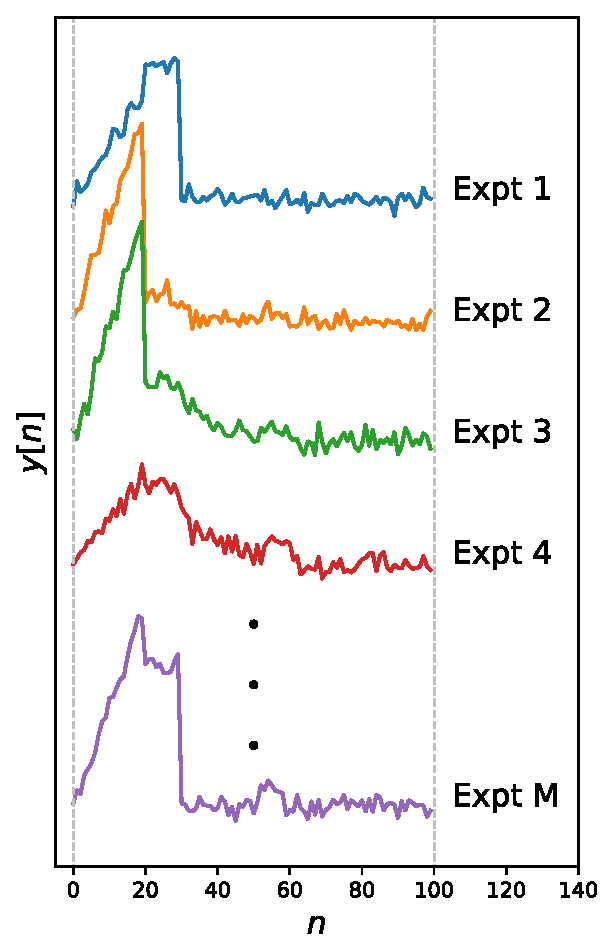
\includegraphics[width=0.7\columnwidth]{sections/figs/trig_expt.eps}
    % \end{center}\vspace{-0.3cm}
    % We know from the physics of the system that the system response to the test signal for the $j^{th}$ experiment given is given by ,
    % \[ y_j\ls n \rs = \sum_{i=1}^{K} w_{ji}\phi_i\ls n\rs + \nu_j\ls n\rs\]
    % where, $n$ is time index; $N$ is the number of data points recorded on each experiment; $\phi_i\ls n\rs, 1 \leq i \leq K$ are characteristic signals of the system; $w_{ji}$ are the weights that determine the amount of the $\phi_i$ present in the output $y_j$ for the $j^{th}$ experiment; and $\nu_j\ls n\rs$ is measurement noise present in the $j^{th}$ experiments. Additionally, we also know that
    % $$ \phi_i^T\phi_j = \sum_{l=0}^{N-1} \phi_i\ls l \rs\phi_j\ls l\rs = \begin{cases} 0 & i \neq j \\ 1 & i = j \end{cases} $$

    % Data from one such experiment is provided in the CSV file (trigexpt.csv) which contains an array of data where the rows correspond to system response for the different experiments, and the columns correspond to  different time index. Using this data identify the different characteristic signals $\phi_i$ for the system, along with the weights $w_{ji}$ for the different experiments. You must also ensure that the data is explained with least number characteristic signal, i.e. $K$ should be as low as possible. Explain how you chose $K$.l
\end{enumerate}

\end{multicols}
\end{document}
% -*- root: ../assignment.tex -*-
\subsection*{Least Squares}
\begin{enumerate}[resume]
    \item The least square approximate solution to  problem $\mf{Ax} = b, \mf{A} \in \mb{R}^{m \times n}$ is obtained by minimizing the following objective fucntion,
    \[ O\lp\mf{x}\rp = \lV\mf{Ax} - \mf{b}\rV^2 = \sum_{i=1}^{m} \lp\tilde{\mf{a}}_i^T\mf{x} - \mf{b}_i\rp^2 \]
    If the the objective function was defined differently, where the different components were given different weights for the different terms, 
    \[ O_w\lp\mf{x}\rp = \sum_{i=1}^{m} w_i\lp\tilde{\mf{a}}_i^T\mf{x} - \mf{b}_i\rp^2 \]
    This is the \textit{weighted least squares}. Find the expression for the approximate solution of the weighted least squares problem.

    \item Consider a matrix $\mf{A} \in \mb{R}^{m \times n}$ with independent columns. There is no matrix $\mf{X}$, such that $\mf{A}\mf{X} = \mf{I}$. Find an expression for the matrix $\mf{X}$, such that $\lV\mf{A}\mf{X} - \mf{I}\rV^2$ is minimum. Hint: Consider the individual columns of $\mf{X}$ and $\mf{I}$.

    \item Consider the following polynomial equation,
    \[ y = \sum_{i=0}^{n} \beta_ix^i, \,\,\,\, x, y, \beta_i \in \mb{R} \]
    This expression is linear in the polynomial coefficients. Fitting a polynomial to data can be done through a linear least square procedure. Conisder a set of measurements $\lc\lp x_l, y_l \rp\rc_{l=1}^{m}$. We are interested in fitting a polynomial that fits this data, such that the difference between the polynomial and data is as low as possible.
    \[ \bmxc y_1\\ y_2\\ \vdots \\ y_m\emxc = \bmxc 1 & x_1 & x_1^2 & \ldots & x_1^n\\ 1 & x_2 & x_2^2 & \ldots & x_2^n\\ \vdots & \vdots & \vdots & \ddots & \vdots\\ 1 & x_m & x_m^2 & \ldots & x_m^n \emxc \bmxc\beta_0 \\ \beta_1 \\ \beta_2 \\ \vdots \\ \beta_n\emxc \]
    \[ \mf{y} = \mf{X}\mf{\beta} \]

    $\mf{X}$ is called the \textit{Vandermonde} matrix. To estimate $\beta$ through a least squares procedure, $\mf{X}$ must have independent columns. Prove that for a set of different $x_i$s the \textit{Vandermonde} matrix has independent columns.

    You are provided with CSV format data file (polyfit.csv) containing data $\lc\lp x_l, y_l \rp\rc_{l=1}^{m}$, to which you are required to fit a polynomial function. The choice of the order of the polynomial is up to you. This can be come from \textit{a priori} knowledge of the system from which data is collected, or it can be decided based on eyeballing the scatter plot between $x_i$ and $y_i$. 

    \begin{enumerate}
        \item \textbf{Data fitting error}: Fit polynomials of orders 0 to 10 to the given data, and for each order determine the data fitting error.
        \[ e_n = \lV\mf{X}\hat{\beta} - \mf{y}\rV \]
        Plot $e_n$ versus the polynomial model order $n$. You should observe the fitting error to monotonically decrease as a function fo $n$. Why is this? Can $e_n$ ever be zero?

        \item \textbf{Model validation}: Even though increasing the polynomial order decreases the data fitting error, this is not always desirable. Given that noise in ubiquitous in all measurements, increasing model order will result in a polynomial that not only fits the general trend in the data, but also the observed measurement noise. Thus, the optimal choice for the model order is determined through a validation procedure, where the data is split into two sets - \textit{training} set and a \textit{testing} set. In order to understand this, you are required to:
        \begin{enumerate}
            \item Split your data $D$ into two sets of size 80\% and 20\%, corresponding to the \textit{training} $D_{train}$ and \textit{testing} $D_{test}$ sets; these percentages are arbitrary. Split you data randomly, such that each data entry is randomly assigned to $D_{train}$ and $D_{test}$.

            \item Fit the polynomial model of a particular order to $D_{train}$. Let the model parameters obtained be $\hat{\beta}$. The validation error for this model is defined as the following.
            \[ e_n^{val} = \lV\mf{X}\hat{\beta} - \mf{y}\rV \]
            where, $\mf{X}$ and $\mf{y}$ comes from the test data set $D_{test}$. Estimate the validation error for different models order 0 to 10, and plot $e_n^{val}$ versus the polynomial model order $n$. How is this plot different from the plot $e_n$ versus $n$? What is the optimal choice for the model order based on the validation procedure?
        \end{enumerate}

        \item \textbf{Regularized data fitting}: Instead of minimzing $\lV\mf{X}\beta - \mf{y}\rV^2$ of the data, now fit a model that minimizes, $\lV\mf{X}\beta - \mf{y}\rV^2 + \lambda\beta^T\beta$, where $\lambda \geq 0$. In this particular case fit the model order to a high value (e.g. 10) and the entire data set $D$. Perform the data ditting procedure for different values of $\lambda$. Plot $\lV\mf{X}\beta - \mf{y}\rV$ verus $\lambda$. Compare the values of $\hat{\beta}$ for the different values of $\lambda$ and compare these to your optimal choice of model parameters from the previous question.
    \end{enumerate}

    \item Consider a time series $\mf{x} = \lc x_0, x_1,\ldots x_{N-1} \rc$ consisting of $N$ data points, where $n$ indicates time index. The time series is corrupted by noise, and we are interested in filtering the time series to obtain a smooth estimate of the the general trend in the time series. This can be posed a problem of estimating a new time series $\hat{\mf{x}}$, such that the difference $\mf{x} - \hat{\mf{x}}$ is minimized and $\hat{\mf{x}}$ is smooth, i.e. the adjacent values of the signal do not change abruptly. 
    \[ O\lp \hat{x} \rp = \sum_{i = 1}^{N} \lp x_i - \hat{x}_i \rp^2 + \lambda \sum_{i = 2}^{N-1} \lp 2 \hat{x}_i - \hat{x}_{i-1} - \hat{x}_{i+1} \rp^2 \]

    If $\mf{x}$ and $\hat{\mf{x}}$ are considered as $N$-vectors, then this can eb written as 
    \[ O\lp \hat{\mf{x}} \rp = \lV \mf{x} - \hat{\mf{x}} \rV^2 + \lambda \lV \mf{D}\hat{\mf{x}} \rV^2 \]

    You are provided with a CSV data file (timeseries.csv) consisting of a time series. Filter this time series by minimizing $O\lp\hat{\mf{x}}\rp$ for different values of $\lambda$. Plot $\mf{x}$ and $\hat{\mf{x}}$ for different values of $\lambda$. What role does $\lambda$ play in the minimzation problem?

    \item Consider the following resistive network, where the horizontal resistors have resistnce of $R_h = 1\Omega$ and the vertical resistors have a resistance of $R_v = 2\Omega$. You goal is to determine a set of currents in the $\mf{i} = \bmx i_1 & i_2 & \ldots & i_{16}\emx^T$, so as to acheive a particular distribution of potentials at the different nodes of the network. Node that we have control only over the currents at the edge nodes, and in the internal nodes the current is zero, i.e. $i_6 = i_7 = i_{10} = i_{11} = 0$.

    \begin{center}
    \begin{circuitikz}[scale=0.8, transform shape]
        \draw (0,0) to[R,*-*] (0,2) to[R,*-*] (0,4) to[R,*-*] (0,6);
        \draw (2,0) to[R,*-*] (2,2) to[R,*-*] (2,4) to[R,*-*] (2,6);
        \draw (4,0) to[R,*-*] (4,2) to[R,*-*] (4,4) to[R,*-*] (4,6);
        \draw (6,0) to[R,*-*] (6,2) to[R,*-*] (6,4) to[R,*-*] (6,6);

        \draw (0,0) to[R,*-*] (2,0) to[R,*-*] (4,0) to[R,*-*] (6,0);
        \draw (0,2) to[R,*-*] (2,2) to[R,*-*] (4,2) to[R,*-*] (6,2);
        \draw (0,4) to[R,*-*] (2,4) to[R,*-*] (4,4) to[R,*-*] (6,4);
        \draw (0,6) to[R,*-*] (2,6) to[R,*-*] (4,6) to[R,*-*] (6,6);

        \draw (-1,7) node[above]{{\Large $i_1$}} to[short, o-] (0,6);
        \draw (2,7) node[above]{{\Large $i_2$}} to[short, o-] (2,6);
        \draw (4,7) node[above]{{\Large $i_3$}} to[short, o-] (4,6);
        \draw (7,7) node[above]{{\Large $i_4$}} to[short, o-] (6,6);

        \draw (7,2) node[right]{{\Large $i_{12}$}} to[short, o-] (6,2);
        \draw (7,4) node[right]{{\Large $i_{5}$}} to[short, o-] (6,4);

        \draw (-1,-1) node[below]{{\Large $i_{16}$}} to[short, o-] (0,0);
        \draw (2,-1) node[below]{{\Large $i_{15}$}} to[short, o-] (2,0);
        \draw (4,-1) node[below]{{\Large $i_{14}$}} to[short, o-] (4,0);
        \draw (7,-1) node[below]{{\Large $i_{13}$}} to[short, o-] (6,0);

        \draw (-1,2) node[left]{{\Large $i_{9}$}} to[short, o-] (0,2);
        \draw (-1,4) node[left]{{\Large $i_{8}$}} to[short, o-] (0,4);

        \draw (0,6) node[below right]{{\large $v_1$}};
        \draw (2,6) node[below right]{{\large $v_2$}};
        \draw (4,6) node[below right]{{\large $v_3$}};
        \draw (6,6) node[below right]{{\large $v_4$}};

        \draw (0,4) node[below right]{{\large $v_8$}};
        \draw (2,4) node[below right]{{\large $v_7$}};
        \draw (4,4) node[below right]{{\large $v_6$}};
        \draw (6,4) node[below right]{{\large $v_5$}};

        \draw (0,2) node[below right]{{\large $v_9$}};
        \draw (2,2) node[below right]{{\large $v_{10}$}};
        \draw (4,2) node[below right]{{\large $v_{11}$}};
        \draw (6,2) node[below right]{{\large $v_{12}$}};

        \draw (0,0) node[below right]{{\large $v_{16}$}};
        \draw (2,0) node[below right]{{\large $v_{15}$}};
        \draw (4,0) node[below right]{{\large $v_{14}$}};
        \draw (6,0) node[above right]{{\large $v_{13}$}};

        \node at (1, 6.5) {$R_h$};
        \node at (-0.6, 5) {$R_v$};
     \end{circuitikz}
     \end{center}

    Let $\mf{v} = \bmx v_1 & v_2 & \ldots & v_{16}\emx$ represent the vector of potential distributions in the network. Then determine $\mf{i}$ such that $\lV\mf{v}_T - \mf{v}\rV^2$ is minimized for the followingdesired potential distribution (Note that the potentias are arragned in a matrix $\mf{V}_{map} = \bmxc 
    v_{1} & v_{2} & v_{3} & v_{4}\\
    v_{8} & v_{7} & v_{6} & v_{5}\\
    v_{9} & v_{10} & v_{11} & v_{12}\\
    v_{16} & v_{15} & v_{14} & v_{13}
    \emxc$
    \begin{enumerate}
        \item $\mf{V}_{map} = \bmxc 
        1 & 2 & 3 & 4\\
        1 & 2 & 3 & 4\\
        1 & 2 & 3 & 4\\
        1 & 2 & 3 & 4
        \emxc $ 
        \item $\mf{V}_{map} = \bmxc 
        2 & 2 & 2 & 2\\
        2 & 1 & 1 & 2\\
        2 & 1 & 1 & 2\\
        2 & 2 & 2 & 2
        \emxc $
        \item $\mf{V}_{map} = \bmxc 
        1 & 1 & 1 & 1\\
        0 & 0 & 0 & 0\\
        0 & 0 & 0 & 0\\
        1 & 1 & 1 & 1
        \emxc $ 
    \end{enumerate}
    for some desired potential distribution $\mf{v}_T$, subject to the constraint $\sum_{k=1}^{16} i_k = 0$.

    \item Trialteration is a process of determining the position $\mf{x} = \bmx x_1 & x_2\emx^T$ of a point $P$ given the distance of the point from a $N$ control points of known locations $\mf{a}_1, \mf{a}_2, \ldots \mf{a}_N$. At any given point in time $n$, we have $N$ different measurements corresponding to the distance of the point $P$ from the $N$ control points, i.e.
    \[ \mf{d}_n = \bmx d_{n1} & d_{n2} & \ldots & d_{nN}\emx^T \]
    where, $d_{ni}^2 = \lV\mf{x}_n - \mf{a}_i\rV_2^2$ for all $1 \leq i \leq N$.
    \begin{center}
    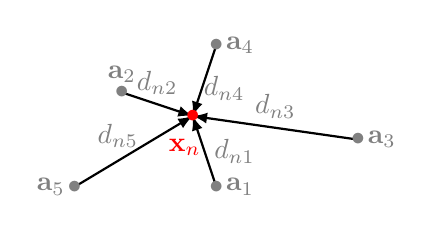
\begin{tikzpicture}[scale=0.6]
        \draw[thick,-latex] (0,0) -- (-0.5, 1.5);
        \node[gray, right] at (-0.25, 0.75) {$d_{n1}$};

        \draw[thick,-latex] (-2,2) -- (-0.5, 1.5);
        \node[gray, above] at (-1.25, 1.75) {$d_{n2}$};

        \draw[thick,-latex] (3,1) -- (-0.5, 1.5);
        \node[gray, above] at (1.25, 1.25) {$d_{n3}$};

        \draw[thick,-latex] (0,3) -- (-0.5, 1.5);
        \node[gray, xshift=0.25cm, yshift=0.2cm] at (-0.25, 1.75) {$d_{n4}$};

        \draw[thick,-latex] (-3,0) -- (-0.5, 1.5);
        \node[gray, xshift=-0.2cm, yshift=0.2cm] at (-1.75, 0.75) {$d_{n5}$};

        \node[gray] at (0,0) {$\bullet$};
        \node[gray, right] at (0,0) {$\mf{a}_1$};
        \node[gray] at (-2,2) {$\bullet$};
        \node[gray, above] at (-2,2) {$\mf{a}_2$};
        \node[gray] at (3,1) {$\bullet$};
        \node[gray, right] at (3,1) {$\mf{a}_3$};
        \node[gray] at (0,3) {$\bullet$};
        \node[gray, right] at (0,3) {$\mf{a}_4$};
        \node[gray] at (-3,0) {$\bullet$};
        \node[gray, left] at (-3,0) {$\mf{a}_5$};
        \node[red] at (-0.5,1.5) {$\bullet$};
        \node[red, xshift=-0.1cm, yshift=-0.1cm] at (-0.5,1) {$\mf{x}_n$};
    \end{tikzpicture}
    \end{center}

    $\mf{x}_n$ are nonlinear functions of the measurements and the control point locations. However, taking the difference between two squared distance measurements $d_j^2$ and $d_i^2$ results in linear equations in the unknown coordinates,
    \[ \lp \mf{a}_i - \mf{a}_j\rp^T\mf{x} = \frac{\lp d_j^2 - \lV\mf{a}_j\rV_2^2 \rp - \lp d_i^2  - \lV\mf{a}_i\rV_2^2 \rp}{2} \]

    Consider the point $P$ that moves with time; $\mf{x}_n \in \mb{R}^{2}$ represents the location of the point at time instant $n$. The distance of this point from a set of 50 different control points is given to you in a CSV data file (trilatdist.csv); the data rows correspond to distance measurements from the different control points at a given point in time, while the colums correpond to the distance of the point from a particular control point for all time. The locations of the 50 control points are available in a separate fileCSV file (trilatctrlpos.csv). Each of these distance measurements is affected by noise. You aim is to use these distance measurements to reconstruct the trajecotry of the point $\mf{x}_n$ as a function of time.
    \begin{enumerate}
        \item What is the minimum number of distance measurements you need to estimate the unknown coordinates of the point $\mf{x}$?
        \item You are provided the actual trajectory of point $P$ in the file trilatactpos.csv. How does you estimate compare with that of the actual trajectory? If we are informed that the point $P$ does not undergo large changes in position between two consecutive time instants $n-1$ and $n$, how would you use this information to improve your estimate?
    \end{enumerate}
\end{enumerate}
% \vfill
% % -*- root: ../assignment.tex -*-
\subsection*{Linear Dynamics Systems -- Transfer function view}
\begin{enumerate}[resume]
    \item Write down the differential equation representing relationship between the loop current $y\ct{t}$ and the input voltage $v\ct{t}$. Assume a initial loop current of $y\ct{0^-} = y_0$.
    \begin{center}
        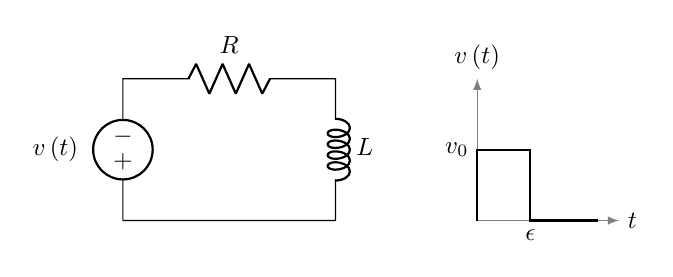
\begin{tikzpicture}[scale=0.9, transform shape]
        \path (0,0) coordinate (ref_gnd);
        \draw
          (ref_gnd) to[american voltage source=$v\lp t\rp$] ++(0,2)
                    to[R=\(R\)] ++(3,0) 
                    to[L=\(L\)] ++(0,-2) 
          -- (ref_gnd);
        
        \draw[-latex, gray] (5, 0) -- (7, 0) node[black, right] {$t$};
        \draw[-latex, gray] (5, 0) -- (5, 2) node[black, above] {$v\ct{t}$};
        \draw[-, black, thick] (5, 0) -- (5, 1) -- (5.75, 1) -- (5.75, 0) -- (6.7, 0);
        \node[black, left] at (5, 1) {$v_0$};
        \node[black, below] at (5.75, 0) {$\epsilon$};
        \end{tikzpicture}
    \end{center}
    \begin{enumerate}
        \item Find the response of the system for the input $v\ct{\bullet}, \forall t \geq 0$ shown in the figure.
        \item Show that for a suitable choice $\epsilon$, $y\ct{t} = 0, \,\, \forall t > \epsilon$.
        \item Assuming $y\ct{0^-} = 0$, what happens to $y\ct{t}$ when, $\epsilon \to 0$ and $v_0 \to \frac{1}{\epsilon}$? Derive the mathematical expression applying this limit. Compare this solution to the input $v\ct{t} = \delta\ct{t}$.
        \item What will happen when $\epsilon \to 0$ and $v_0$ is constant?  
    \end{enumerate}

    \item Derive the differential equation governing the following two mechanical systems. The input to both these systems is the force $f\ct{t}$, and the position $x\ct{t}$ is the output; assume the initial conditions to $x\ct{0^-}, \dot{x}\ct{0^-}$.

    \begin{center}
    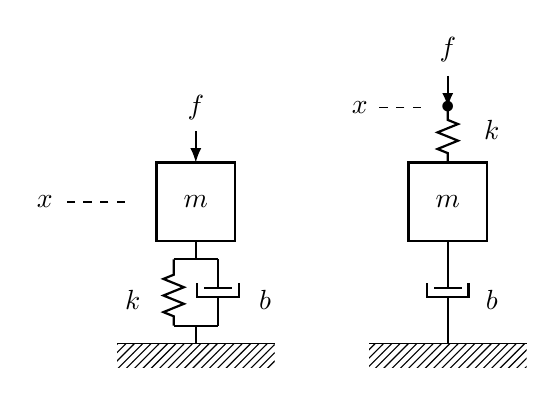
\begin{tikzpicture}[every node/.style={draw,outer sep=0pt,thick}, scale=0.8]
    %define the spring
    \tikzstyle{spring}=[thick,decorate,decoration={zigzag,pre length=0.12cm,post length=0.12cm,amplitude=1.3mm,segment length=6}]

    %define the dashpot
    \tikzstyle{damper}=[thick,decoration={markings,
      mark connection node=dmp,
      mark=at position 0.5 with 
      {
          \node (dmp) [thick,inner sep=0pt,transform shape,rotate=-90,minimum width=15pt,minimum height=3pt,draw=none] {};    
          \draw [thick] ($(dmp.north east)+(2pt,0)$) -- (dmp.south east) -- (dmp.south west) -- ($(dmp.north west)+(2pt,0)$);
          \draw [thick] ($(dmp.north)+(0,-5pt)$) -- ($(dmp.north)+(0,5pt)$);
      }
    }, decorate]

    %define the spring-dashpot
    \tikzstyle{spr-dash}=[thick,decorate,decoration={markings,
      mark connection node=sqr,
      mark=at position 0.5 with
      {
          \node (sqr) [thick,minimum width=16pt,minimum height=24pt,draw=none] {};
          \draw [thick] (sqr.north west) -- (sqr.north east);
          \draw [thick] (sqr.south west) -- (sqr.south east);
          \draw [spring] (sqr.south west) -- (sqr.north west);
          \draw [damper] (sqr.south east) -- (sqr.north east);
      }
      }]

    %define the ground
    \tikzstyle{ground}=[fill,pattern=north east lines,draw=none, minimum width=0.75cm, minimum height=0.3cm]

    %define node stype
    \tikzset{simplenode/.append style={draw=none}}

    \begin{scope}[xshift=0.0cm]
    %draw the frame mass
    \node (M1) [minimum width=1cm,minimum height=1cm] {$m$};
    
    \node (ground-medium) at (M1.south) [ground,yshift=-1.3cm,minimum width=2cm,anchor=north] {};
    \draw (ground-medium.north west) -- (ground-medium.north east);

    \draw [spr-dash] (ground-medium.north) -- (M1.south);
    \node [draw=none] at ($(ground-medium.north)+(-1cm,0.7cm)$) {$k$};
    \node [draw=none] at ($(ground-medium.north)+(1.1cm,0.7cm)$) {$b$};

    \draw [dashed,thin] (M1.west) ++ (-0.5cm, 0) -- +(-1.0cm, 0);
    \node [draw=none, left] at ($(M1.west) + (-1.5cm, 0cm)$) {$x$};

    \draw [-latex,thick] (M1.north) ++ (0, 0.5cm) -- (M1.north);
    \node [draw=none, yshift=0.7cm] at (M1.north) {$f$};
    \end{scope}

    \begin{scope}[xshift=4.0cm]
    %draw the frame mass
    \node (M1) [minimum width=1cm,minimum height=1cm] {$m$};
    \node (ground-medium) at (M1.south) [ground,yshift=-1.3cm,minimum width=2cm,anchor=north] {};
    \draw (ground-medium.north west) -- (ground-medium.north east);

    \draw [damper] (ground-medium.north) -- (M1.south);
    \draw [spring] (M1.north) -- (0, 1.5cm);
    \node [draw=none] at ($(ground-medium.north)+(0.7cm,3.4cm)$) {$k$};
    \node [draw=none] at ($(ground-medium.north)+(0.7cm,0.7cm)$) {$b$};

    \draw [dashed,thin] (M1.west) ++ (0.2cm, 1.5) -- +(-0.75cm, 0);
    \node [draw=none, left] at ($(M1.west) + (-0.5cm, 1.5cm)$) {$x$};

    \draw [-latex,thick] (0, 2.0cm) -- (0, 1.5cm);
    \node[simplenode] at (0, 1.5cm) {$\bullet$};
    \node [draw=none, yshift=0.1cm] at (0, 2.3) {$f$};
    \end{scope}
    \end{tikzpicture}
    \end{center}

    Find the expression for the step response of these two systems. 

    \item Consider a continuous-time LTI system with impulse response, $h\ct{t} = e^{-2t}1\ct{t}$. What is the output of this system to the following inputs using the convolution integral?
    \begin{enumerate*}
        \item $e^{-2t}1\ct{t}$;
        \item $e^{-2t}$;
        \item $e^{-1t}$;
        \item $e^{-4t}$; and 
        \item $\cos\ct{\omega t}$.
    \end{enumerate*}

    Now, obtain the expression for the output of the system for the above inputs using the system's transfer function $H\ct{s}$.

    \item Find the impulse response and transfer functions of the following composition of subsystems with individual impulse response $h_i\ct{t}$.
    \begin{center}
        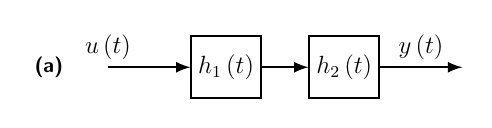
\begin{tikzpicture}[scale=0.75, transform shape, thick, node distance=2cm]
        \draw
            node [input, name=input1] {} 
            node [block, right of=input1] (sys1) {{\large $h_1\ct{t}$}}
            node [block, right of=sys1] (sys2) {{\large $h_2\ct{t}$}}
            node [input, right of=sys2, name=output1] {};
            \draw[-latex] node [above] {{\large $u\ct{t}$}} (input1) -- node {} (sys1);
            \draw[-latex](sys1) -- node {} (sys2);
            \draw[-latex](sys2) -- node[above] {\large $y\ct{t}$} (output1);
            \node[]  at (-1,0) {\textbf{(a)}};
        \end{tikzpicture}

        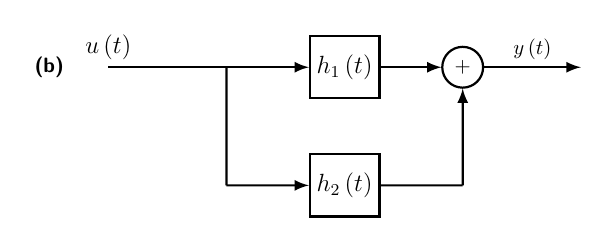
\begin{tikzpicture}[scale=0.75, transform shape, thick, node distance=2cm]
        \draw
            node [input, name=input1] {}
            node [input, right of=input1, name=tempin1] {} 
            node [input, below of=tempin1, name=tempin2] {} 
            node [block, right of=tempin1] (sys1) {{\large $h_1\ct{t}$}}
            node [block, right of=tempin2] (sys2) {{\large $h_2\ct{t}$}}
            node [sum, right of=sys1] (suma1) {$\suma$} 
            node [input, right of=sys2, name=tempout2] {}
            node [input, right of=suma1, name=output1] {};

            \draw[-] node [above] {{\large $u\ct{t}$}} (input1) -- node {} (tempin1);
            \draw[-latex] node {} (tempin1) -- node {} (sys1);
            \draw[-] node {} (tempin1) -- node {} (tempin2);
            \draw[-latex] node {} (tempin2) -- node {} (sys2);
            \draw[-latex](sys1) -- (suma1);
            \draw[-] node {} (sys2) -- node {} (tempout2);
            \draw[-latex] node {} (tempout2) -- node {} (suma1);
            \draw[-latex] node {} (suma1) -- node[above] {$y\ct{t}$} (output1);
            \node[]  at (-1,0) {\textbf{(b)}};
        \end{tikzpicture}

        \begin{tikzpicture}[scale=0.75, transform shape, thick, node distance=2cm]
        \draw
            node [input, name=input1] {}
            node [sum, right of=input1] (suma1) {$\suma$} 
            node [input, below of=suma1, name=tempfb] {} 
            node [block, right of=suma1] (sys1) {{\large $h_1\ct{t}$}}
            node [input, right of=sys1, name=tempout1] {}
            node [input, right of=tempout1, name=output1] {}
            node [input, below of=tempout1, name=tempout2] {}
            node [block, below of=sys1] (sys2) {{\large $h_2\ct{t}$}};

            \draw[-latex] node [above] {{\large $u\ct{t}$}} (input1) -- node {} (suma1);
            \draw[-latex] node {} (suma1) -- node {} (sys1);
            \draw[-] node {} (sys1) -- node {} (tempout1);
            \draw[-latex] node {} (tempout1) -- node {} (output1);
            \draw[-] node {} (tempout1) -- node {} (tempout2);
            \draw[-latex] node {} (tempout2) -- node {} (sys2);
            \draw[-] node {} (sys2) -- node {} (tempin2);
            \draw[-latex] node {} (tempin2) -- node {} (suma1);
            \node[]  at (-1,0) {\textbf{(c)}};
        \end{tikzpicture}
    \end{center}

    \item Consider the second order system, $\ddot{y}\ct{t} + 2\zeta\omega_n\dot{y}\ct{t} + \omega_n^2y\ct{t} = u\ct{t}$. Find the impulse response of this system. Plot the impulse response of the system for $\omega_n = 1$ and the following values of the parameter $\zeta$.
    \begin{enumerate*}
        \item $\zeta = \sqrt{2}$;
        \item $\zeta = 1$;
        \item $\zeta = 0.5$;
        \item $\zeta = 0$;
        \item $\zeta = -0.5$; and 
        \item $\zeta = -1.0$;
    \end{enumerate*}
    For each of these parameter values show the location of the poles of the corresponding transfer function.
\end{enumerate}
% \vfill
% % -*- root: ../assignment.tex -*-
\subsection*{Linear Dynamics Systems -- State space view}
\begin{enumerate}[resume]
    \item Derive the state and measurement equations for the following composite systems, assuming the system $H_i$ to have the parameters $\ct{\mf{A}_i, \mf{B}_i, \mf{C}_i, \mf{D}_i}$.
    \begin{center}
        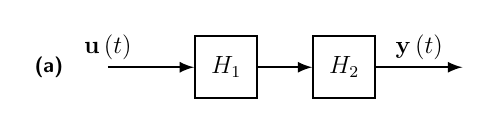
\begin{tikzpicture}[scale=0.75, transform shape, thick, node distance=2cm]
        \draw
            node [input, name=input1] {} 
            node [block, right of=input1] (sys1) {{\large $H_1$}}
            node [block, right of=sys1] (sys2) {{\large $H_2$}}
            node [input, right of=sys2, name=output1] {};
            \draw[-latex] node [above] {{\large $\mf{u}\ct{t}$}} (input1) -- node {} (sys1);
            \draw[-latex](sys1) -- node {} (sys2);
            \draw[-latex](sys2) -- node[above] {\large $\mf{y}\ct{t}$} (output1);
            \node[]  at (-1,0) {\textbf{(a)}};
        \end{tikzpicture}

        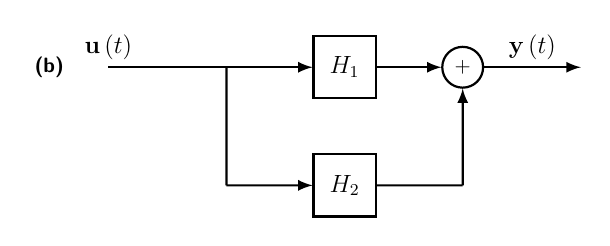
\begin{tikzpicture}[scale=0.75, transform shape, thick, node distance=2cm]
        \draw
            node [input, name=input1] {}
            node [input, right of=input1, name=tempin1] {} 
            node [input, below of=tempin1, name=tempin2] {} 
            node [block, right of=tempin1] (sys1) {{\large $H_1$}}
            node [block, right of=tempin2] (sys2) {{\large $H_2$}}
            node [sum, right of=sys1] (suma1) {$\suma$} 
            node [input, right of=sys2, name=tempout2] {}
            node [input, right of=suma1, name=output1] {};

            \draw[-] node [above] {{\large $\mf{u}\ct{t}$}} (input1) -- node {} (tempin1);
            \draw[-latex] node {} (tempin1) -- node {} (sys1);
            \draw[-] node {} (tempin1) -- node {} (tempin2);
            \draw[-latex] node {} (tempin2) -- node {} (sys2);
            \draw[-latex](sys1) -- (suma1);
            \draw[-] node {} (sys2) -- node {} (tempout2);
            \draw[-latex] node {} (tempout2) -- node {} (suma1);
            \draw[-latex] node {} (suma1) -- node[above] {\large $\mf{y}\ct{t}$} (output1);
            \node[]  at (-1,0) {\textbf{(b)}};
        \end{tikzpicture}

        \begin{tikzpicture}[scale=0.75, transform shape, thick, node distance=2cm]
        \draw
            node [input, name=input1] {}
            node [sum, right of=input1] (suma1) {$\suma$} 
            node [input, below of=suma1, name=tempfb] {} 
            node [block, right of=suma1] (sys1) {{\large $H_1$}}
            node [input, right of=sys1, name=tempout1] {}
            node [input, right of=tempout1, name=output1] {}
            node [input, below of=tempout1, name=tempout2] {}
            node [block, below of=sys1] (sys2) {{\large $H_2$}};

            \draw[-latex] node [above] {{\large $\mf{u}\ct{t}$}} (input1) -- node {} (suma1);
            \draw[-latex] node {} (suma1) -- node {} (sys1);
            \draw[-] node {} (sys1) -- node {} (tempout1);
            \draw[-latex] node {} (tempout1) -- node {} (output1);
            \draw[-] node {} (tempout1) -- node {} (tempout2);
            \draw[-latex] node {} (tempout2) -- node {} (sys2);
            \draw[-] node {} (sys2) -- node {} (tempin2);
            \draw[-latex] node {} (tempin2) -- node {} (suma1);
            \draw[-latex] node {} (tempout1) -- node[above] {\large $\mf{y}\ct{t}$} (output1);
            \node[]  at (-1,0) {\textbf{(c)}};
        \end{tikzpicture}
    \end{center}
    
    \item Derive the state and measurement equation for the following system, where the input is the force $f$ applied to mass $m_2$, and the output is the acceleration of the mass $m_1$ and velocity of mass $m_2$.
    \begin{center}
    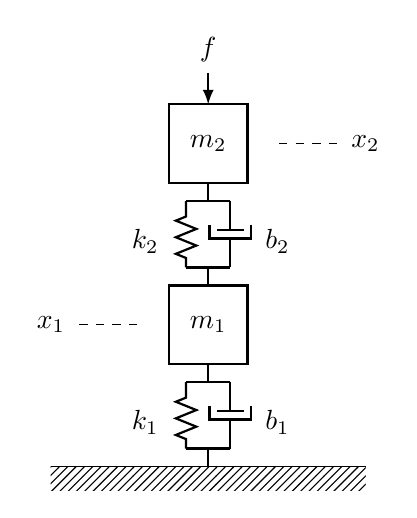
\begin{tikzpicture}[every node/.style={draw,outer sep=0pt,thick}, scale=0.8]
    %define the spring
    \tikzstyle{spring}=[thick,decorate,decoration={zigzag,pre length=0.12cm,post length=0.12cm,amplitude=1.3mm,segment length=6}]

    %define the dashpot
    \tikzstyle{damper}=[thick,decoration={markings,
      mark connection node=dmp,
      mark=at position 0.5 with 
      {
          \node (dmp) [thick,inner sep=0pt,transform shape,rotate=-90,minimum width=15pt,minimum height=3pt,draw=none] {};    
          \draw [thick] ($(dmp.north east)+(2pt,0)$) -- (dmp.south east) -- (dmp.south west) -- ($(dmp.north west)+(2pt,0)$);
          \draw [thick] ($(dmp.north)+(0,-5pt)$) -- ($(dmp.north)+(0,5pt)$);
      }
    }, decorate]

    %define the spring-dashpot
    \tikzstyle{spr-dash}=[thick,decorate,decoration={markings,
      mark connection node=sqr,
      mark=at position 0.5 with
      {
          \node (sqr) [thick,minimum width=16pt,minimum height=24pt,draw=none] {};
          \draw [thick] (sqr.north west) -- (sqr.north east);
          \draw [thick] (sqr.south west) -- (sqr.south east);
          \draw [spring] (sqr.south west) -- (sqr.north west);
          \draw [damper] (sqr.south east) -- (sqr.north east);
      }
      }]

    %define the ground
    \tikzstyle{ground}=[fill,pattern=north east lines,draw=none,minimum width=0.75cm,minimum height=0.3cm]

    \begin{scope}[xshift=5.5cm]
    %draw the frame mass
    \node (M1) [minimum width=1cm,minimum height=1cm] {$m_1$};
     
    %draw the vehicle mass
    \node (M2) at (M1.north) [yshift=+1.8cm, minimum width=1cm, minimum height=1cm] {$m_2$};

    \node (ground-medium) at (M1.south) [ground,yshift=-1.3cm,minimum width=4cm,anchor=north] {};
    \draw (ground-medium.north west) -- (ground-medium.north east);

    \draw [spr-dash] (ground-medium.north) -- (M1.south);
    \node [draw=none] at ($(ground-medium.north)+(-1cm,0.7cm)$) {$k_{1}$};
    \node [draw=none] at ($(ground-medium.north)+(1.1cm,0.7cm)$) {$b_{1}$};
    \draw [spr-dash] (M1.north) -- (M2.south);
    \node [draw=none] at ($(M1.north)+(-1.0cm,0.7cm)$) {$k_{2}$};
    \node [draw=none] at ($(M1.north)+(1.1cm,0.7cm)$) {$b_{2}$};
     
    \draw [-latex,thick] (M2.north) ++ (0, 0.5cm) -- (M2.north);
    \draw [dashed,thin] (M2.east) ++ (0.5cm, 0) -- +(1.0cm, 0);
    \node [draw=none, right] at ($(M2.east) + (1.5cm, 0)$) {$x_{2}$};

    \draw [dashed,thin] (M1.west) ++ (-0.5cm, 0) -- +(-1.0cm, 0);
    \node [draw=none, left] at ($(M1.west) + (-1.5cm, 0cm)$) {$x_{1}$};

    \node [draw=none, yshift=0.7cm] at (M2.north) {$f$};
    \end{scope}
    \end{tikzpicture}
    \end{center}

    Assume now that instead of $f$ the input to this was the position of the mass $m_2$ (i.e. $x_2$) and the output of interest was the acceleration of the mass $m_1$. What would be correspondoing state and measurement equations in this case?

    \item Obtain a state space representation for the following systems:
    \begin{enumerate}
        \item $\sum_{i=0}^n a_iy^{\ct{i}} = \sum_{j=0}^m b_jx^{\ct{j}}$, where $x^{\ct{k}} = \frac{d^k}{dt^k}x\ct{t}$
        \item $\sum_{i=0}^n a_iy\dt{k+i} = \sum_{j=0}^m b_jx\dt{k+j}$
    \end{enumerate}

    \item Write down the state and measurement equations for the following system with the scalar input $u\dt{k}$ and output $\mf{y}\dt{k} = \bmx y_1\dt{k}\\ y_2\dt{k}\emx$. 

    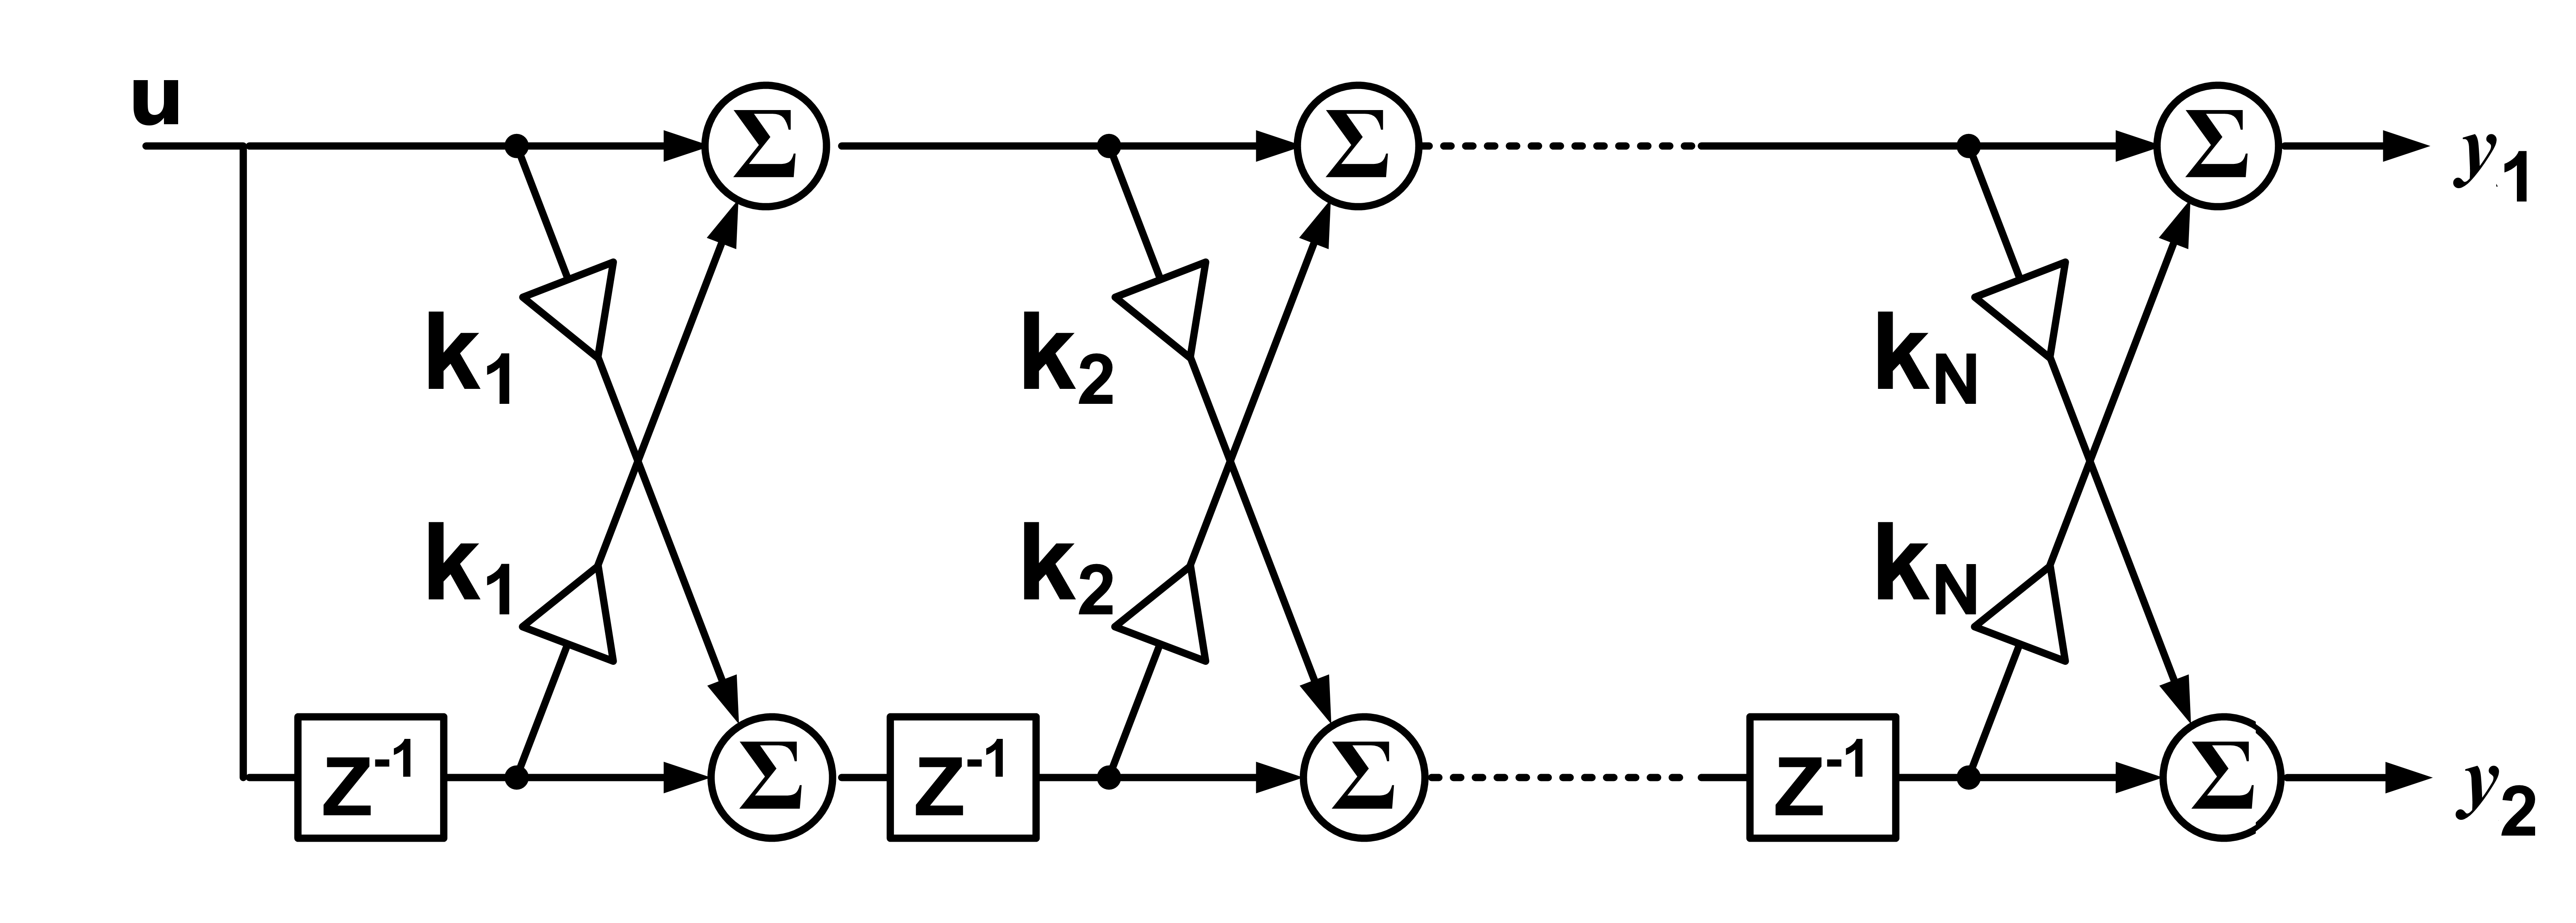
\includegraphics[width=0.45\textwidth]{sections/figs/latticefilt.png}

    \item The following model shows two media and their constituent elements. Medium 1 consists of elements with mass $M_1$ which are interconnected through a spring and damper in parallel with spring constant $k_1$ and damping coefficient $b_1$. Medium 2 consits of elements with mass $M_2$ connected through $k_2$ and $b_2$. At the interface $M_1$ and $M_2$ are connected through $k_3$ nd $b_3$.

    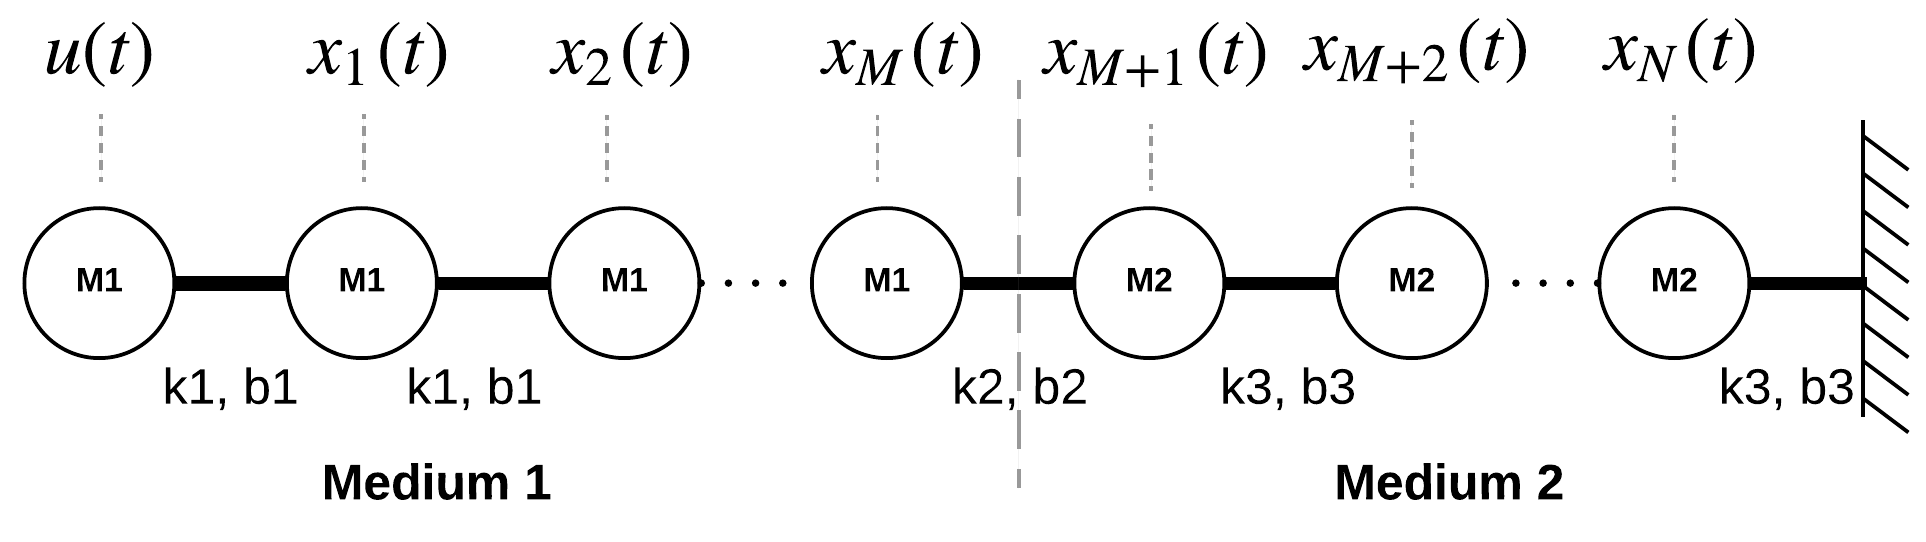
\includegraphics[width=0.45\textwidth]{sections/figs/wavetx.png}    

    The input to this system is $u\ct{t}$ which is the position imposed on the let most element in medium 1. The output of the system are the successive differences in the positions of the massess.
    \[ y_i\ct{t} = x_{i+2}\ct{t} - x_{i+1}\ct{t} \, ,\,\,\, 1 \leq i \leq N-2 \]

    Derive the state and measurement equations for the system.


\end{enumerate}
% \vfill
% % -*- root: ../assignment.tex -*-
% \subsection*{Solution of LDS}
\begin{enumerate}[resume]
    \item Consider $\mf{A} = \bmx 1 & 1 & 0\\ 0 & 0 & 1\\ 0 & 0 & 1\emx$. Compute $\mf{A}^{100}$ and $e^{t\mf{A}}$.

    \item Assuming that $\mf{A} \in \mb{R}^{n \times n}$ is diagonalizable with eigenvalues $\lambda_1, \lambda_2,\ldots \lambda_n$. Prove that the eigenvalues of $e^{\mf{A}}$ are $e^{\lambda_1}, e^{\lambda_2}, \ldots e^{\lambda_n}$

    \item Consider a linear time-variant discrete-time, $\mf{x}\dt{k+1} = \mf{A}\dt{k}\mf{x}\dt{k} + \mf{B}\dt{k}\mf{u}\dt{k}$. Find the general expression for the zero-input solution, and the zero-state solution.

    \item What are the conditions on the individual LTI discrete-time systems $H_1\ct{z}$ and $H_2\ct{z}$ for the following overall system to be:
    \begin{enumerate*}
        \item internally stable;
        \item externally stable;
        \item controllable; and
        \item observable
    \end{enumerate*}
    \begin{center}
        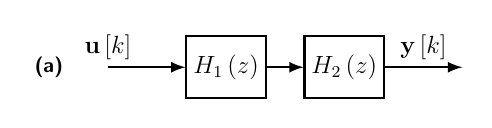
\begin{tikzpicture}[scale=0.75, transform shape, thick, node distance=2cm]
        \draw
            node [input, name=input1] {} 
            node [block, right of=input1] (sys1) {{\large $H_1\ct{z}$}}
            node [block, right of=sys1] (sys2) {{\large $H_2\ct{z}$}}
            node [input, right of=sys2, name=output1] {};
            \draw[-latex] node [above] {{\large $\mf{u}\dt{k}$}} (input1) -- node {} (sys1);
            \draw[-latex](sys1) -- node {} (sys2);
            \draw[-latex](sys2) -- node[above] {\large $\mf{y}\dt{k}$} (output1);
            \node[]  at (-1,0) {\textbf{(a)}};
        \end{tikzpicture}

        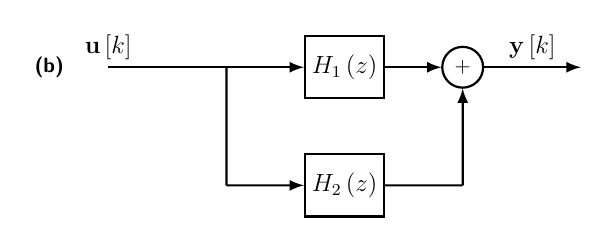
\begin{tikzpicture}[scale=0.75, transform shape, thick, node distance=2cm]
        \draw
            node [input, name=input1] {}
            node [input, right of=input1, name=tempin1] {} 
            node [input, below of=tempin1, name=tempin2] {} 
            node [block, right of=tempin1] (sys1) {{\large $H_1\ct{z}$}}
            node [block, right of=tempin2] (sys2) {{\large $H_2\ct{z}$}}
            node [sum, right of=sys1] (suma1) {$\suma$} 
            node [input, right of=sys2, name=tempout2] {}
            node [input, right of=suma1, name=output1] {};

            \draw[-] node [above] {{\large $\mf{u}\dt{k}$}} (input1) -- node {} (tempin1);
            \draw[-latex] node {} (tempin1) -- node {} (sys1);
            \draw[-] node {} (tempin1) -- node {} (tempin2);
            \draw[-latex] node {} (tempin2) -- node {} (sys2);
            \draw[-latex](sys1) -- (suma1);
            \draw[-] node {} (sys2) -- node {} (tempout2);
            \draw[-latex] node {} (tempout2) -- node {} (suma1);
            \draw[-latex] node {} (suma1) -- node[above] {\large $\mf{y}\dt{k}$} (output1);
            \node[]  at (-1,0) {\textbf{(b)}};
        \end{tikzpicture}

        % \begin{tikzpicture}[scale=0.75, transform shape, thick, node distance=2cm]
        % \draw
        %     node [input, name=input1] {}
        %     node [sum, right of=input1] (suma1) {$\suma$} 
        %     node [input, below of=suma1, name=tempfb] {} 
        %     node [block, right of=suma1] (sys1) {{\large $H_1$}}
        %     node [input, right of=sys1, name=tempout1] {}
        %     node [input, right of=tempout1, name=output1] {}
        %     node [input, below of=tempout1, name=tempout2] {}
        %     node [block, below of=sys1] (sys2) {{\large $H_2$}};

        %     \draw[-latex] node [above] {{\large $\mf{u}\ct{t}$}} (input1) -- node {} (suma1);
        %     \draw[-latex] node {} (suma1) -- node {} (sys1);
        %     \draw[-] node {} (sys1) -- node {} (tempout1);
        %     \draw[-latex] node {} (tempout1) -- node {} (output1);
        %     \draw[-] node {} (tempout1) -- node {} (tempout2);
        %     \draw[-latex] node {} (tempout2) -- node {} (sys2);
        %     \draw[-] node {} (sys2) -- node {} (tempin2);
        %     \draw[-latex] node {} (tempin2) -- node {} (suma1);
        %     \draw[-latex] node {} (tempout1) -- node[above] {\large $\mf{y}\ct{t}$} (output1);
        %     \node[]  at (-1,0) {\textbf{(c)}};
        % \end{tikzpicture}
    \end{center}

    \item Consider a the LTI system, $\dot{\mf{x}}\ct{t} = \mf{A}\mf{x}\ct{t}$, where $\mf{A} \in \mb{R}^{n \times n}$. An experiment was carried out with this system, where the system was started at different initial conditions $\mf{x}_i\ct{0^-}$, and the corresponding state trajectories were recorded to be $\mf{x}_i\ct{t}, \,\, \forall t \geq 0$. Assuming that the set of initial conditions$\lc \mf{x}\ct{0^-} \rc_{i=1}^n$ are linearly independent, find the expression for the $e^{t\mf{A}}$.

    \item Consider the following system, where the input is the force $f$ applied to mass $m_2$, and the output of the system, positions of masses $m_1$ and $m_2$, are measured using a set of position sensors. 
    \begin{enumerate}
        \item Is this system controllable? Is the system still controllable if the input $f$ was acting on the mass $m_1$ instead of $m_2$?
        \item Is this system observable? If instead of measuring both position $x_1$ and $x_2$, if the output of the system was either $x_1$ or $x_2$, is the system still observable?
    \end{enumerate}
    \begin{center}
    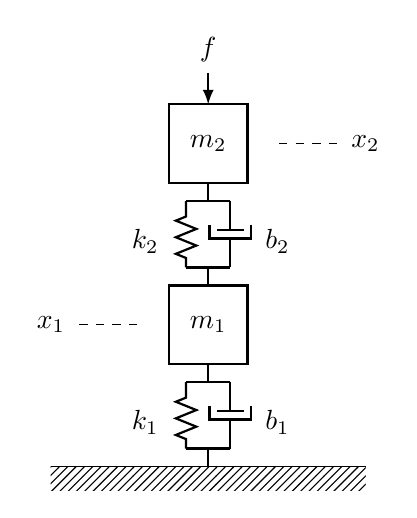
\begin{tikzpicture}[every node/.style={draw,outer sep=0pt,thick}, scale=0.8]
    %define the spring
    \tikzstyle{spring}=[thick,decorate,decoration={zigzag,pre length=0.12cm,post length=0.12cm,amplitude=1.3mm,segment length=6}]

    %define the dashpot
    \tikzstyle{damper}=[thick,decoration={markings,
      mark connection node=dmp,
      mark=at position 0.5 with 
      {
          \node (dmp) [thick,inner sep=0pt,transform shape,rotate=-90,minimum width=15pt,minimum height=3pt,draw=none] {};    
          \draw [thick] ($(dmp.north east)+(2pt,0)$) -- (dmp.south east) -- (dmp.south west) -- ($(dmp.north west)+(2pt,0)$);
          \draw [thick] ($(dmp.north)+(0,-5pt)$) -- ($(dmp.north)+(0,5pt)$);
      }
    }, decorate]

    %define the spring-dashpot
    \tikzstyle{spr-dash}=[thick,decorate,decoration={markings,
      mark connection node=sqr,
      mark=at position 0.5 with
      {
          \node (sqr) [thick,minimum width=16pt,minimum height=24pt,draw=none] {};
          \draw [thick] (sqr.north west) -- (sqr.north east);
          \draw [thick] (sqr.south west) -- (sqr.south east);
          \draw [spring] (sqr.south west) -- (sqr.north west);
          \draw [damper] (sqr.south east) -- (sqr.north east);
      }
      }]

    %define the ground
    \tikzstyle{ground}=[fill,pattern=north east lines,draw=none,minimum width=0.75cm,minimum height=0.3cm]

    \begin{scope}[xshift=5.5cm]
    %draw the frame mass
    \node (M1) [minimum width=1cm,minimum height=1cm] {$m_1$};
     
    %draw the vehicle mass
    \node (M2) at (M1.north) [yshift=+1.8cm, minimum width=1cm, minimum height=1cm] {$m_2$};

    \node (ground-medium) at (M1.south) [ground,yshift=-1.3cm,minimum width=4cm,anchor=north] {};
    \draw (ground-medium.north west) -- (ground-medium.north east);

    \draw [spr-dash] (ground-medium.north) -- (M1.south);
    \node [draw=none] at ($(ground-medium.north)+(-1cm,0.7cm)$) {$k_{1}$};
    \node [draw=none] at ($(ground-medium.north)+(1.1cm,0.7cm)$) {$b_{1}$};
    \draw [spr-dash] (M1.north) -- (M2.south);
    \node [draw=none] at ($(M1.north)+(-1.0cm,0.7cm)$) {$k_{2}$};
    \node [draw=none] at ($(M1.north)+(1.1cm,0.7cm)$) {$b_{2}$};
     
    \draw [-latex,thick] (M2.north) ++ (0, 0.5cm) -- (M2.north);
    \draw [dashed,thin] (M2.east) ++ (0.5cm, 0) -- +(1.0cm, 0);
    \node [draw=none, right] at ($(M2.east) + (1.5cm, 0)$) {$x_{2}$};

    \draw [dashed,thin] (M1.west) ++ (-0.5cm, 0) -- +(-1.0cm, 0);
    \node [draw=none, left] at ($(M1.west) + (-1.5cm, 0cm)$) {$x_{1}$};

    \node [draw=none, yshift=0.7cm] at (M2.north) {$f$};
    \end{scope}
    \end{tikzpicture}
    \end{center}

    % Assume now that instead of $f$ the input to this was the position of the mass $m_2$ (i.e. $x_2$) and the output of interest was the acceleration of the mass $m_1$. What would be correspondoing state and measurement equations in this case?

    % \item Obtain a state space representation for the following systems:
    % \begin{enumerate}
    %     \item $\sum_{i=0}^n a_iy^{\ct{i}} = \sum_{j=0}^m b_jx^{\ct{j}}$, where $x^{\ct{k}} = \frac{d^k}{dt^k}x\ct{t}$
    %     \item $\sum_{i=0}^n a_iy\dt{k+i} = \sum_{j=0}^m b_jx\dt{k+j}$
    % \end{enumerate}

    % \item Write down the state and measurement equations for the following system with the scalar input $u\dt{k}$ and output $\mf{y}\dt{k} = \bmx y_1\dt{k}\\ y_2\dt{k}\emx$. 

    % 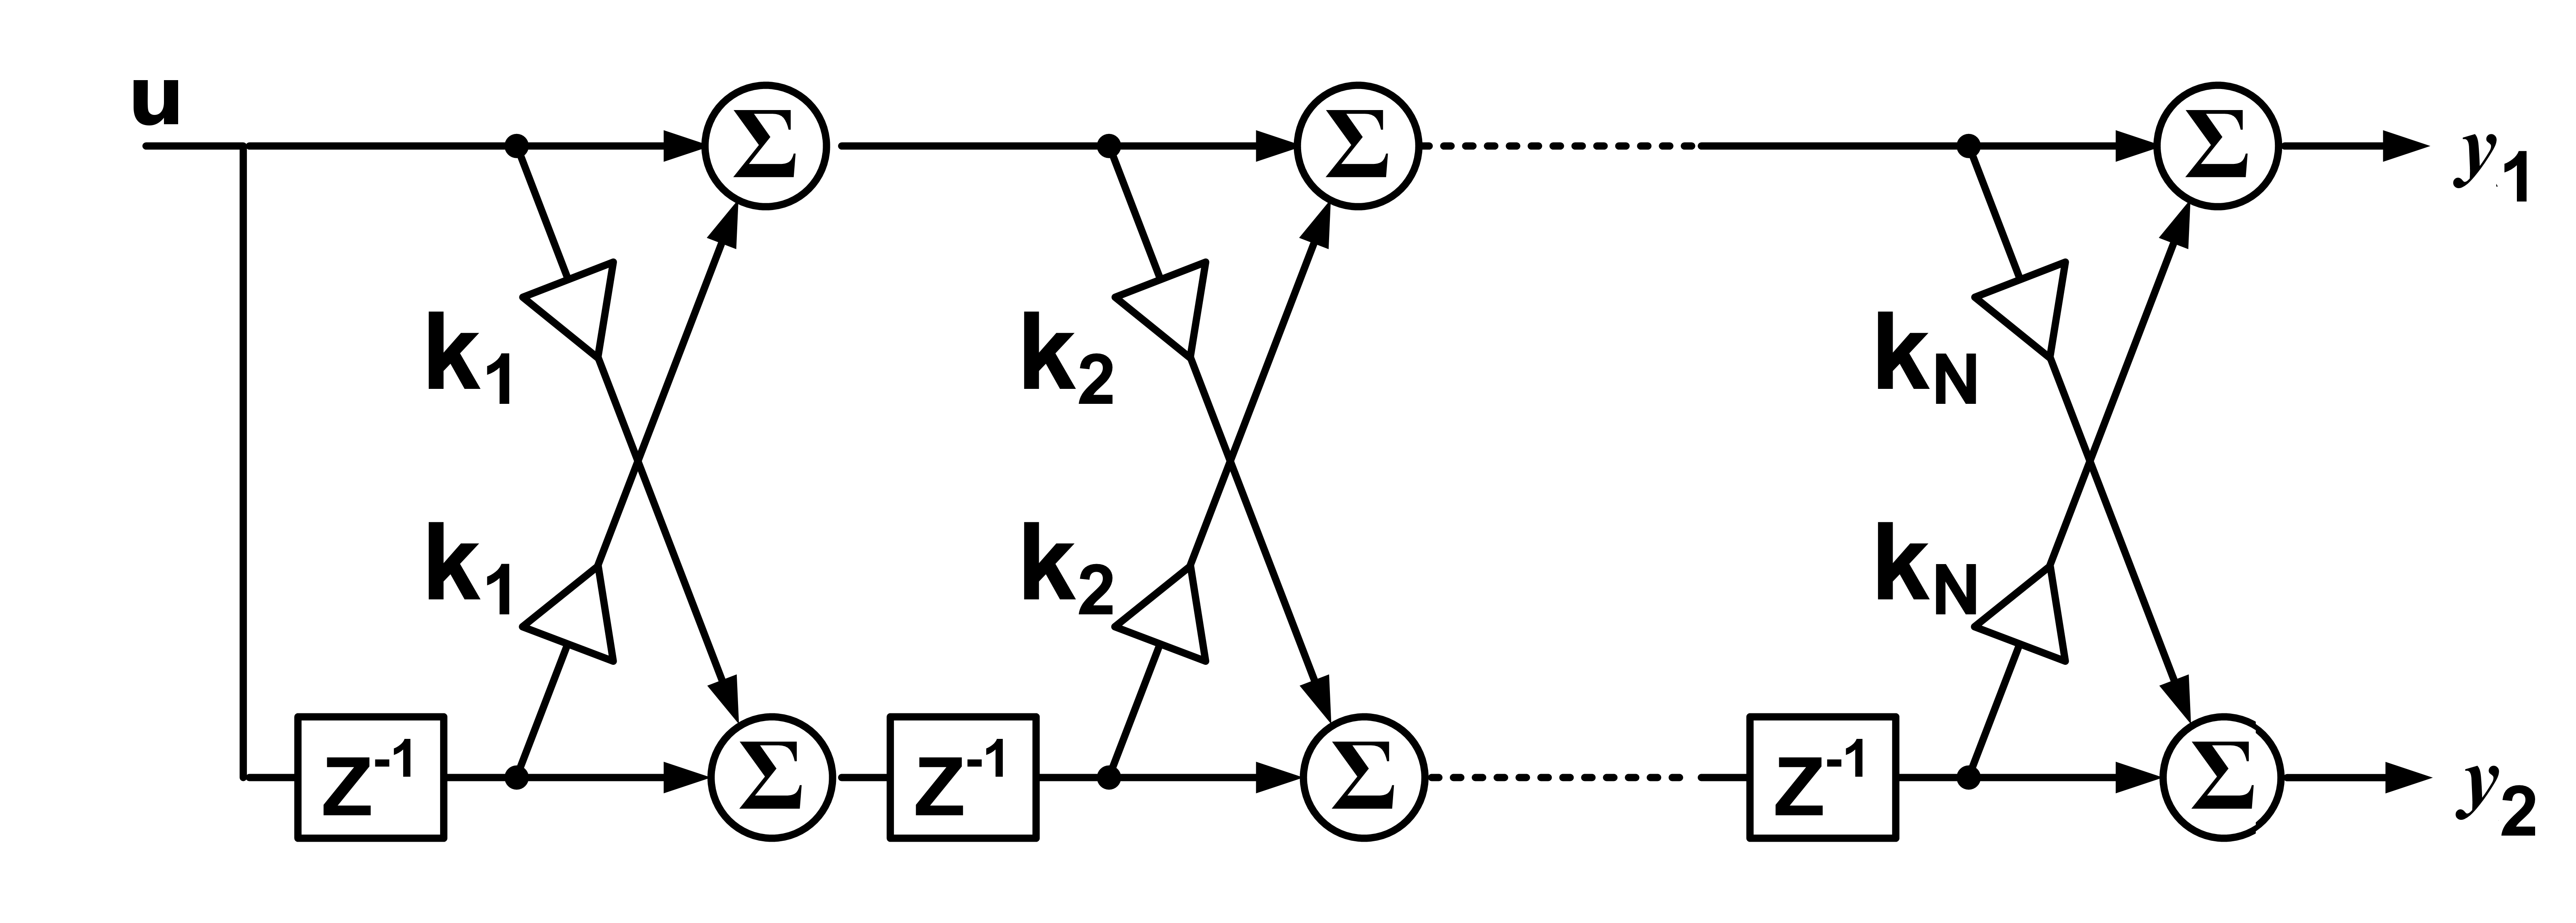
\includegraphics[width=0.45\textwidth]{sections/figs/latticefilt.png}

    % \item The following model shows two media and their constituent elements. Medium 1 consists of elements with mass $M_1$ which are interconnected through a spring and damper in parallel with spring constant $k_1$ and damping coefficient $b_1$. Medium 2 consits of elements with mass $M_2$ connected through $k_2$ and $b_2$. At the interface $M_1$ and $M_2$ are connected through $k_3$ nd $b_3$.

    % 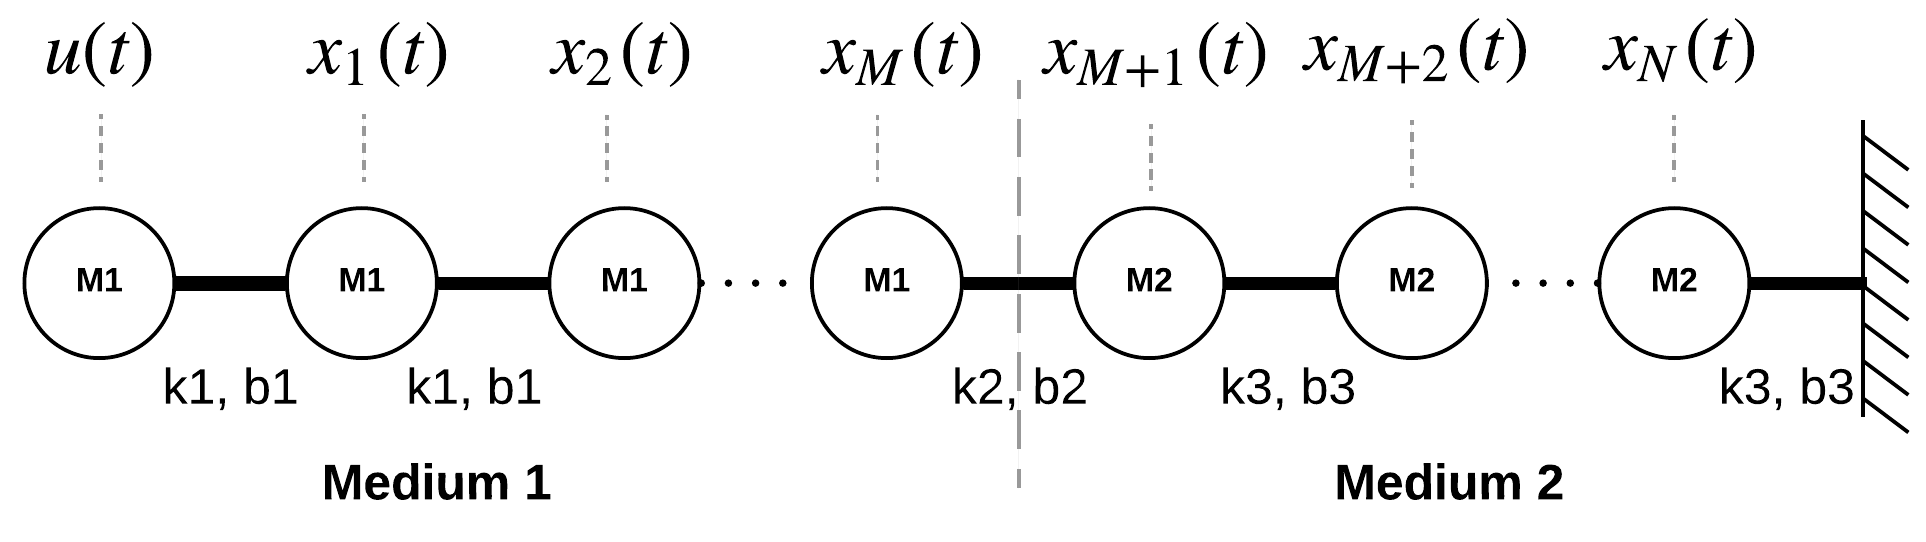
\includegraphics[width=0.45\textwidth]{sections/figs/wavetx.png}    

    % The input to this system is $u\ct{t}$ which is the position imposed on the let most element in medium 1. The output of the system are the successive differences in the positions of the massess.
    % \[ y_i\ct{t} = x_{i+2}\ct{t} - x_{i+1}\ct{t} \, ,\,\,\, 1 \leq i \leq N-2 \]

    % Derive the state and measurement equations for the system.


\end{enumerate}
% \vfill

\newpage
\begin{thebibliography}{50}
\bibitem{strang} G. Strang \textsl{Introduction to linear algebra}.
Wellesley-Cambridge Press Wellesley, MA, USA, 1993
\end{thebibliography}

\end{multicols}
\end{document}